%%%%%%%%%%%%%%%%%%%%%%%%%%%%%%%%%%%%%%%%%%%%%%%%%%%%%%%%%%%%%%%%%%%%%%%%%%%%%%%%%%%%%%%%%%%%%%%%%%%
%%%%%%%%%%%%%%%%%%%%%%%%%%%%%%%%%%%%%%%%%%%%%%%%%%%%%%%%%%%%%%%%%%%%%%%%%%%%%%%%%%%%%%%%%%%%%%%%%%%
%%%%%%%%%%%%%%%%%%%%%%%%%%%%%%%%%%%%%%%%%%%%%%%%%%%%%%%%%%%%%%%%%%%%%%%%%%%%%%%%%%%%%%%%%%%%%%%%%%%
%%%%%%%%%%%%%%%%%%%%%%%%%%%%%%%%%%%%%%%%%%%%%%%%%%%%%%%%%%%%%%%%%%%%%%%%%%%%%%%%%%%%%%%%%%%%%%%%%%%

\chapter{Tablas}

Se incluyen las gráficas y tablas para cada participante en el estudio; por simplicidad, en el 
texto los datos son resumidos por grupos y junto algunos ejemplos.

En las primeras tres tablas (\ref{total_gpos_total}, \ref{total_gpos_mor}) se reporta el número 
total de épocas clasificadas como estacionarias, por cada participante y canal, y con especial
atención al sueño MOR.

Posteriormente, en la tabla \ref{comparacion_mor_vs_total}, se muestran las diferencias 
signitficativas encontradas al comparar la proporción de épocas estacionarias durante las etapas 
MOR y NMOR; este análisis se hizo usando la prueba $\chi^{2}$ para proporciones.

%%%%%%%%%%%%%%%%%%%%%%%%%%%%%%%%%%%%%%%%%%%%%%%%%%%%%%%%%%%%%%%%%%%%%%%%%%%%%%%%%%%%%%%%%%%%%%%%%%%

\begin{SidewaysTable}
\centering
\begin{tabular}{c}
\textbf{Épocas estacionarias en todo el registro}
\vspace{1em}
\end{tabular}
\begin{tabular}{lrrrrrcrrrrcrrr}
\toprule
& \multicolumn{5}{c}{{Gpo. Control}} && 
  \multicolumn{4}{c}{{Gpo. PDC}} && 
  \multicolumn{3}{c}{{Excluidos}}\\
\cmidrule{2-6} \cmidrule{8-11} \cmidrule{13-15}
& {VCR} & {MJH} & {JAE} & {GHA} & {MFGR} & \phantom{l}
& {CLO} & {RLO} & {RRU} & {JGZ} & \phantom{l}
& {FGH} & {MGG} & {EMT} \\
\midrule
{C3} &193&153&110&176&124&&61 &188&92 &57 &&18&229&500 \\
{C4} &175&145&93 &158&97 &&40 &175&99 &47 &&8&230&624 \\
{CZ} &169&147&101&109&85 &&59 &167&73 &63 &&9&193&537 \\
\rowcolor{gris}
{F3} &173&157&93 &150&76 &&64 &218&82 &71 &&113&157&351 \\
\rowcolor{gris}
{F4} &191&155&60 &147&25 &&47 &171&85 &49 &&0&141&573 \\
\rowcolor{gris}
{F7} &163&152&79 &213&91 &&46 &130&68 &58 &&0&154&286 \\
\rowcolor{gris}
{F8} &161&134&36 &169&39 &&45 &119&87 &48 &&0&130&594 \\
{FP1}&165&82 &24 &128&66 &&34 &0  &72 &44 &&403&169&540 \\
{FP2}&157&88 &47 &116&23 &&34 &114&27 &44 &&0&147&467 \\
{FZ} &181&152&97 &156&57 &&62 &201&93 &67 &&0&197&556 \\
\rowcolor{gris}
{O1} &212&194&56 &298&198&&50 &175&101&98 &&25&158&694 \\
\rowcolor{gris}
{O2} &179&188&66 &250&194&&35 &170&79 &107&&23&173&589 \\
{P3} &181&139&55 &290&158&&77 &180&116&95 &&30&236&507 \\
{P4} &184&155&112&257&158&&60 &162&115&74 &&22&221&516 \\
{PZ} &160&146&95 &219&134&&61 &199&116&59 &&16&185&517 \\
\rowcolor{gris}
{T3} &191&169&53 &238&197&&91 &146&84 &102&&29&144&634 \\
\rowcolor{gris}
{T4} &193&141&37 &185&149&&29 &145&118&88 &&10&132&548 \\
\rowcolor{gris}
{T5} &228&172&16 &268&226&&83 &171&109&63 &&21&239&640 \\
\rowcolor{gris}
{T6} &233&166&52 &209&201&&41 &142&102&86 &&18&218&577 \\
{LOG}&242&244&222&287&179&&149&196&130&225&&51&445&850 \\
{ROG}&242&226&229&336&170&&135&186&114&226&&67&474&906 \\
{EMG}&108&73 &16 &1  &174&&34 &98 &114&10 &&1&58&273 \\
\rowcolor{gris}
{Total}&861&1032&907&1093&822&&944&846&414&1207&&405&1030&1423 \\
\bottomrulec
\end{tabular}
\caption{Total de épocas clasificadas como estacionarias. En la 
última fila el total de épocas registradas.
}
\label{total_gpos_total}
\end{SidewaysTable}

%%%%%%%%%%%%%%%%%%%%%%%%%%%%%%%%%%%%%%%%%%%%%%%%%%%%%%%%%%%%%%%%%%%%%%%%%%%%%%%%%%%%%%%%%%%%%%%%%%%

\begin{SidewaysTable}
\centering
\begin{tabular}{c}
\textbf{Épocas estacionarias durante sueño MOR (R)}
\vspace{1em}
\end{tabular}
\begin{tabular}{lrrrrrcrrrrcrrr}
\toprule
& \multicolumn{5}{c}{{Grupo NN}} && 
  \multicolumn{4}{c}{{Gporupo MN}} && 
  \multicolumn{3}{c}{{Excluidos}}\\
\cmidrule{2-6} \cmidrule{8-11} \cmidrule{13-15}
& {VCR} & {MJH} & {JAE} & {GHA} & {MFGR} & \phantom{l}
& {CLO} & {RLO} & {RRU} & {JGZ} & \phantom{l}
& {FGH} & {MGG} & {EMT} \\
\midrule
{C3} &6 &18&10&1 &12&&6 &35&16&1 &&2 &28&22 \\
{C4} &7 &16&4 &2 &10&&4 &40&5 &0 &&1 &23&26 \\
{CZ} &2 &16&13&2 &8 &&5 &22&4 &1 &&1 &13&19 \\
\rowcolor{gris}
{F3} &5 &23&10&0 &3 &&7 &43&3 &3 &&6 &14&20 \\
\rowcolor{gris}
{F4} &11&23&5 &1 &1 &&6 &36&5 &0 &&0 &4 &24 \\
\rowcolor{gris}
{F7} &5 &15&2 &0 &4 &&1 &18&0 &0 &&0 &2 &24 \\
\rowcolor{gris}
{F8} &4 &11&6 &1 &3 &&4 &23&1 &0 &&0 &2 &20 \\
{FP1}&2 &7 &1 &0 &1 &&0 &0 &1 &0 &&22&0 &22 \\
{FP2}&1 &6 &3 &0 &2 &&1 &15&1 &0 &&0 &1 &18 \\
{FZ} &11&18&19&0 &6 &&7 &38&2 &2 &&0 &20&23 \\
\rowcolor{gris}
{O1} &10&20&5 &3 &23&&2 &25&9 &2 &&5 &18&19 \\
\rowcolor{gris}
{O2} &13&23&3 &3 &21&&3 &34&9 &1 &&1 &12&16 \\
{P3} &6 &17&2 &2 &26&&5 &33&8 &0 &&1 &24&17 \\
{P4} &4 &19&4 &5 &18&&4 &27&5 &1 &&4 &15&21 \\
{PZ} &4 &15&5 &3 &22&&4 &32&4 &0 &&1 &8 &20 \\
\rowcolor{gris}
{T3} &10&29&1 &8 &26&&10&34&4 &0 &&2 &29&31 \\
\rowcolor{gris}
{T4} &12&20&2 &3 &21&&3 &35&6 &1 &&0 &10&17 \\
\rowcolor{gris}
{T5} &10&26&0 &3 &27&&5 &34&5 &2 &&2 &31&19 \\
\rowcolor{gris}
{T6} &15&18&3 &15&20&&3 &24&4 &2 &&0 &9 &19 \\
{LOG}&6 &20&8 &0 &9 &&5 &11&2 &0 &&1 &8 &30 \\
{ROG}&6 &21&17&2 &11&&9 &7 &4 &1 &&0 &19&33 \\
{EMG}&14&11&0 &0 &17&&14&16&4 &0 &&0&3&7 \\
\rowcolor{gris}
{Total}&73&127&171&55&95&&132&99&38&33&&22&166&47 \\
\bottomrulec
\end{tabular}
\caption{Total de épocas en sueño MOR clasificadas como estacionarias. En la 
última fila el total de épocas en sueño MOR.
}
\label{total_gpos_mor}
\end{SidewaysTable}

%%%%%%%%%%%%%%%%%%%%%%%%%%%%%%%%%%%%%%%%%%%%%%%%%%%%%%%%%%%%%%%%%%%%%%%%%%%%%%%%%%%%%%%%%%%%%%%%%%%

\begin{SidewaysTable}
\centering
\bordes{1.1}
\begin{tabular}{c}
{Comparación individual para proporción de épocas PE, MOR vs NMOR}
\vspace{1em}
\end{tabular}
\begin{tabular}{lrrrrrcrrrrcrrr}
\toprule
& \multicolumn{5}{c}{{Gpo. Control}} && 
  \multicolumn{4}{c}{{Gpo. PDC}} && 
  \multicolumn{3}{c}{{Excluidos}}\\
\cmidrule{2-6} \cmidrule{8-11} \cmidrule{13-15}
& {VCR} & {MJH} & {JAE} & {GHA} & {MFGR} & \phantom{l}
& {CLO} & {RLO} & {RRU} & {JGZ} & \phantom{l}
& {FGH} & {MGG} & {EMT} \\
\midrule 
{C3} &** & &*  &** &  &&   &** &*  & && & &  \\
{C4} &*  & &***&*  &  &&   &***&   & && &*&  \\
{CZ} &***& &   &   &  &&   &   &   & && &***&  \\
\rowcolor{gris}
{F3} &** & &   &** &  &&   &***&   & && &*&** \\
\rowcolor{gris}
{F4} &   & &   &*  &  &&   &***&   & && &***&  \\
\rowcolor{gris}
{F7} &*  & &***&***&  &&   &   &*  & && &***&*** \\
\rowcolor{gris}
{F8} &** & &   &** &  &&   &*  &*  & && &***&  \\
{FP1}&***& &   &*  &* &&   &   &*  & && &***&  \\
{FP2}&***& &   &*  &  &&   &   &   & && &***&  \\
{FZ} &   & &   &***&  &&   &***&*  & && &*&  \\
\rowcolor{gris}
{O1} &*  & &   &***&  &&   &   &   & &&*& &  \\
\rowcolor{gris}
{O2} &   & &*  &***&  &&   &***&   & && &***& \\ 
{P3} &*  & &*  &***&  &&   &** &   & && &*&  \\
{P4} &***& &***&*  &  &&   &   &   & &&*&***&  \\
{PZ} &** & &***&*  &  &&   &   &*  & && &***&  \\
\rowcolor{gris}
{T3} &   & &** &   &  &&   &***&   & && & &** \\
\rowcolor{gris}
{T4} &   & &   &*  &  &&   &***&   & && &*&  \\
\rowcolor{gris}
{T5} &*  & &   &***&  &&   &***&   & && & &  \\
\rowcolor{gris}
{T6} &   & &*  &   &  &&   &   &   & && &***&  \\
{LOG}&***& &***&***&**&&***&** &***&*&& &***&  \\
{ROG}&***& &***&***&* &&*  &***&*  &*&& &***&  \\
{EMG}&   & &   &   &  &&***&   &*  & && & &  \\
\rowcolor{gris}
{General}& & & & & &&***& &*& && & & \\
\bottomrulec
\end{tabular}
\caption{Diferencias significativas para la comparación entre proporción de épocas PE en
sueño MOR y NMOR; los asteriscos representan el p-valor con el cual se rechaza la hipótesis 
de igualdad: *=0.05 , **=0.01 , ***=0.005}
\label{comparacion_mor_vs_total}
\end{SidewaysTable}

%%%%%%%%%%%%%%%%%%%%%%%%%%%%%%%%%%%%%%%%%%%%%%%%%%%%%%%%%%%%%%%%%%%%%%%%%%%%%%%%%%%%%%%%%%%%%%%%%%%
%%%%%%%%%%%%%%%%%%%%%%%%%%%%%%%%%%%%%%%%%%%%%%%%%%%%%%%%%%%%%%%%%%%%%%%%%%%%%%%%%%%%%%%%%%%%%%%%%%%

\chapter{Compilados gráficos}

En este apéndice se muestran los compilados gráficos mencionados en la parte de resultados,
y que representan la
distribución temporal y pseudo-espacial de las ocurrencia de épocas PSG dentro de los registros 
para cada paciente. 

Primeramente se presentan los compilados gráficos en los que se ha destacado el sueño MOR;
posteriormente se presentan los mismos gráficos resaltando los patrones visuales
propuestos, que parecen estar relacionados con la aparición de sueño MOR.

\begin{figure}
\centering
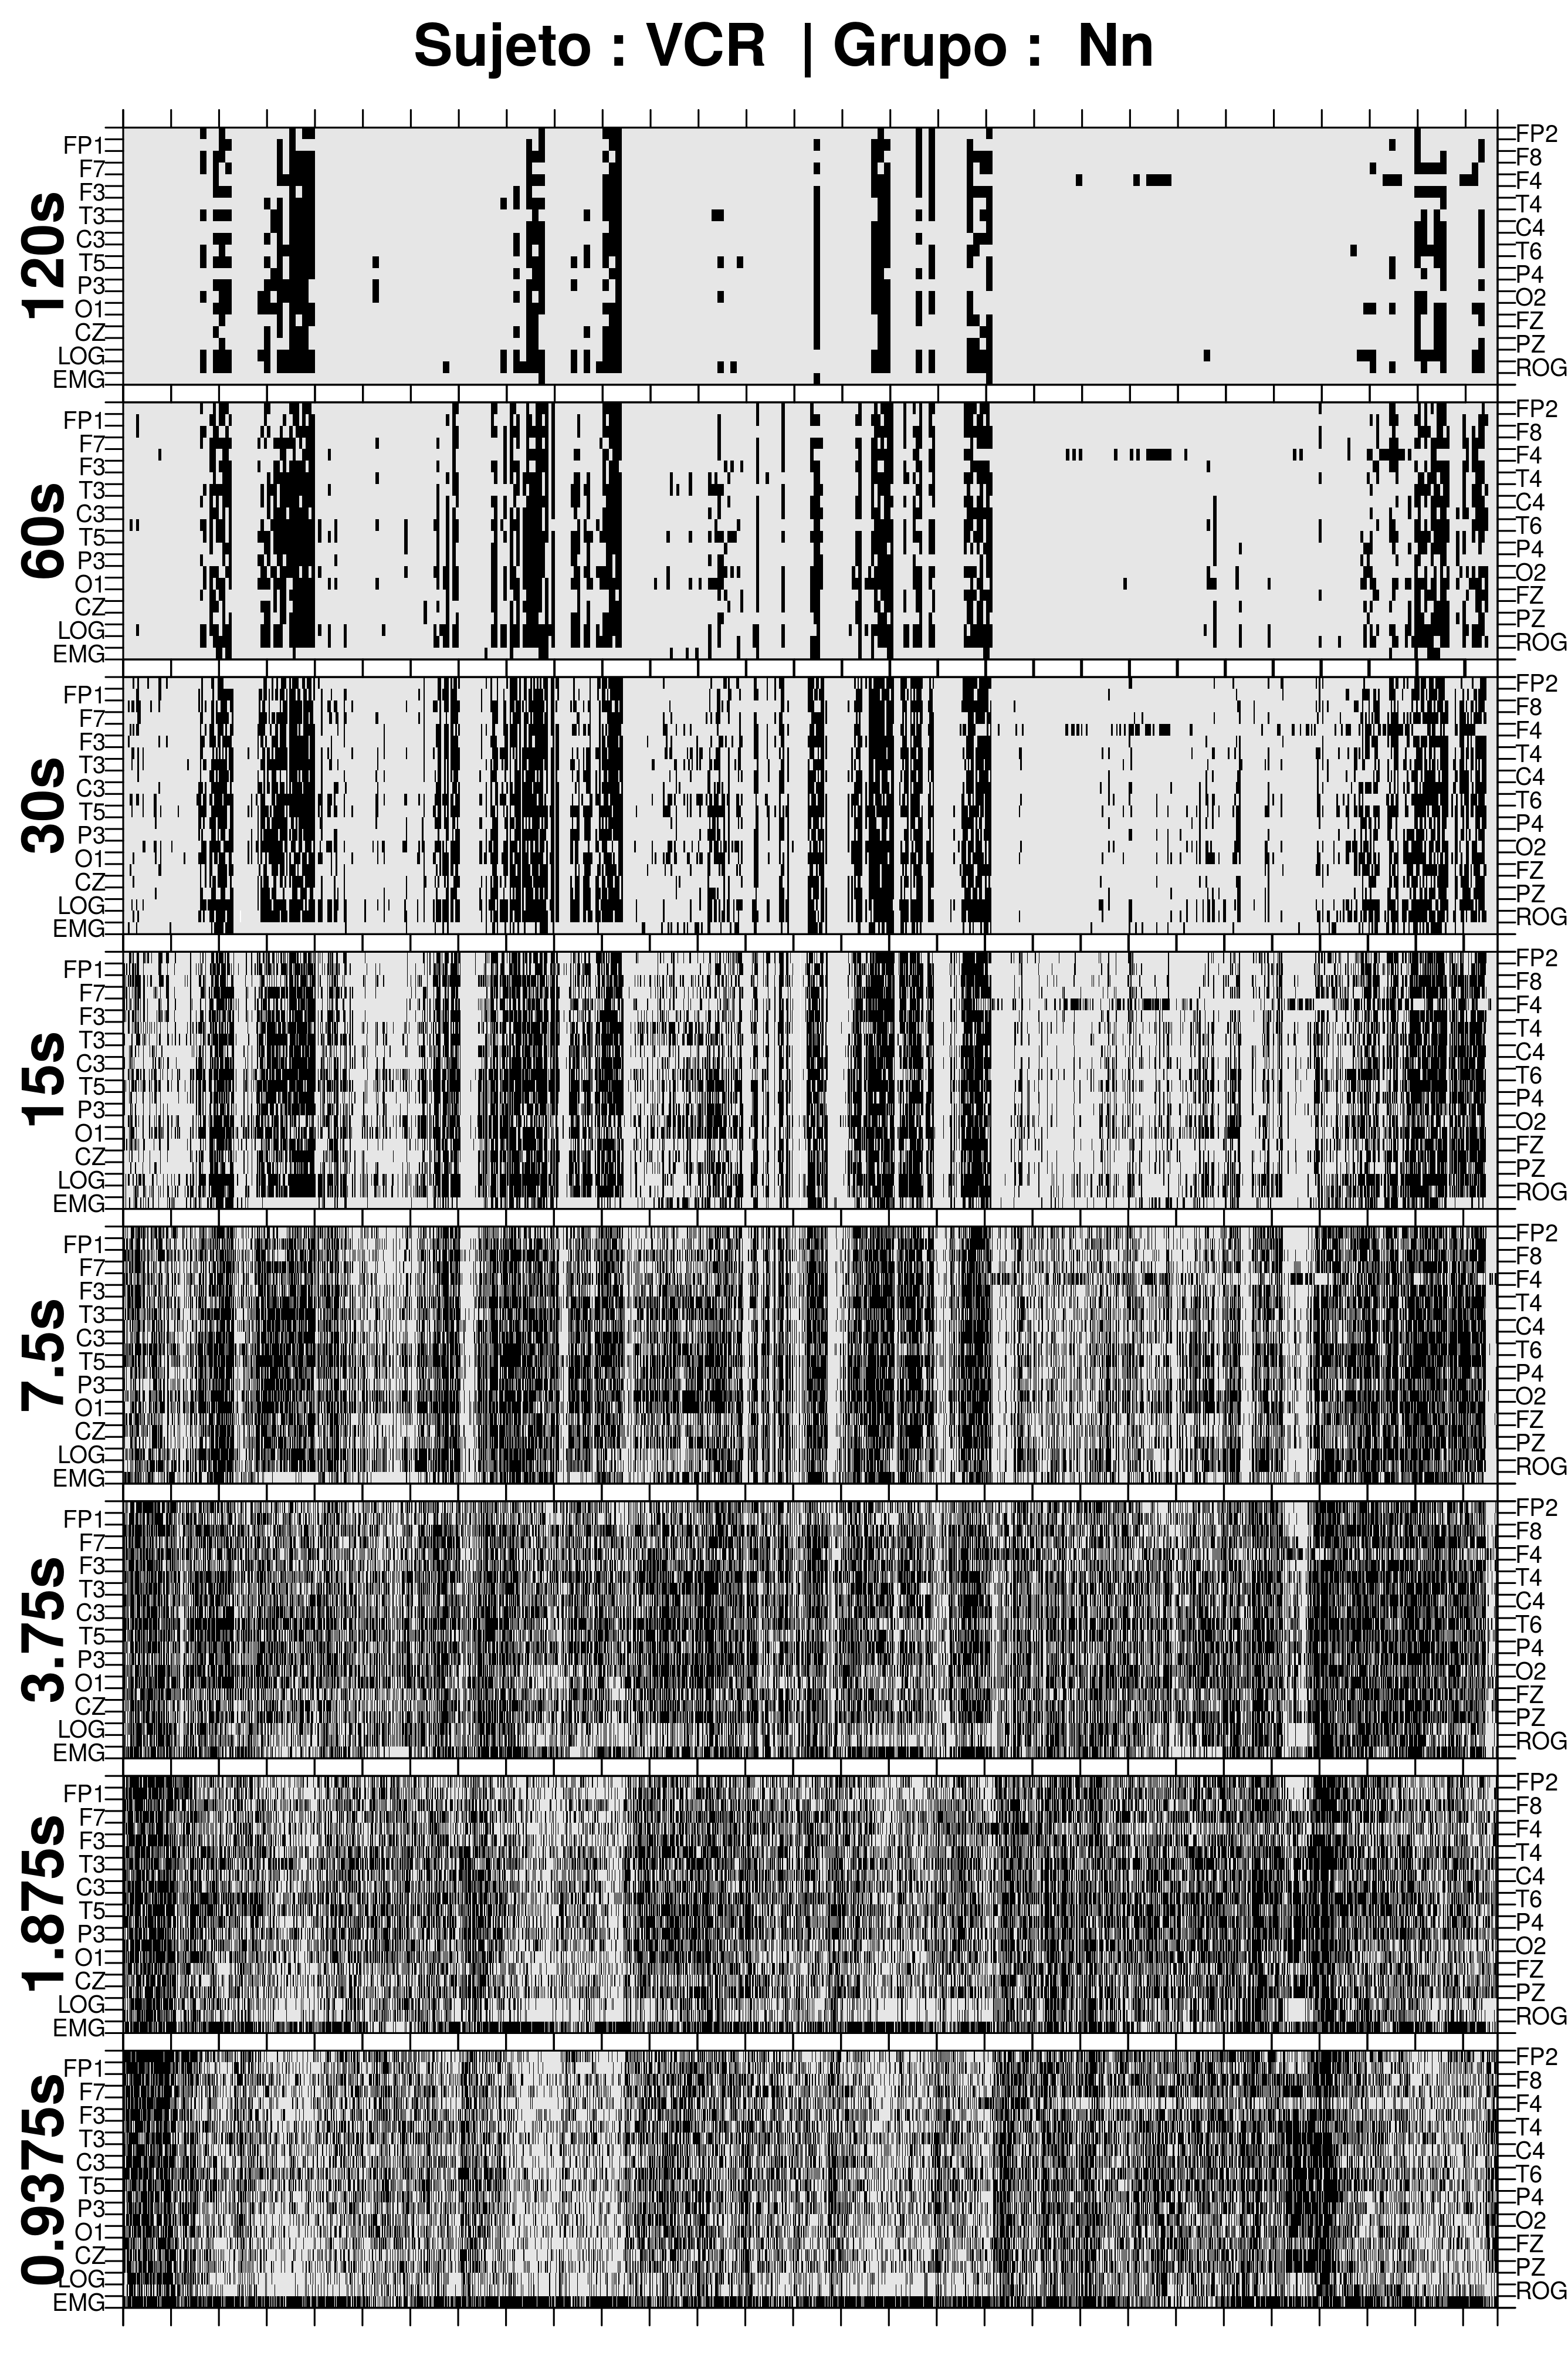
\includegraphics[width=0.9\linewidth]
{./img_ejemplos/VCNNS1_comp_est_.png} 
\end{figure}

\begin{figure}
\centering
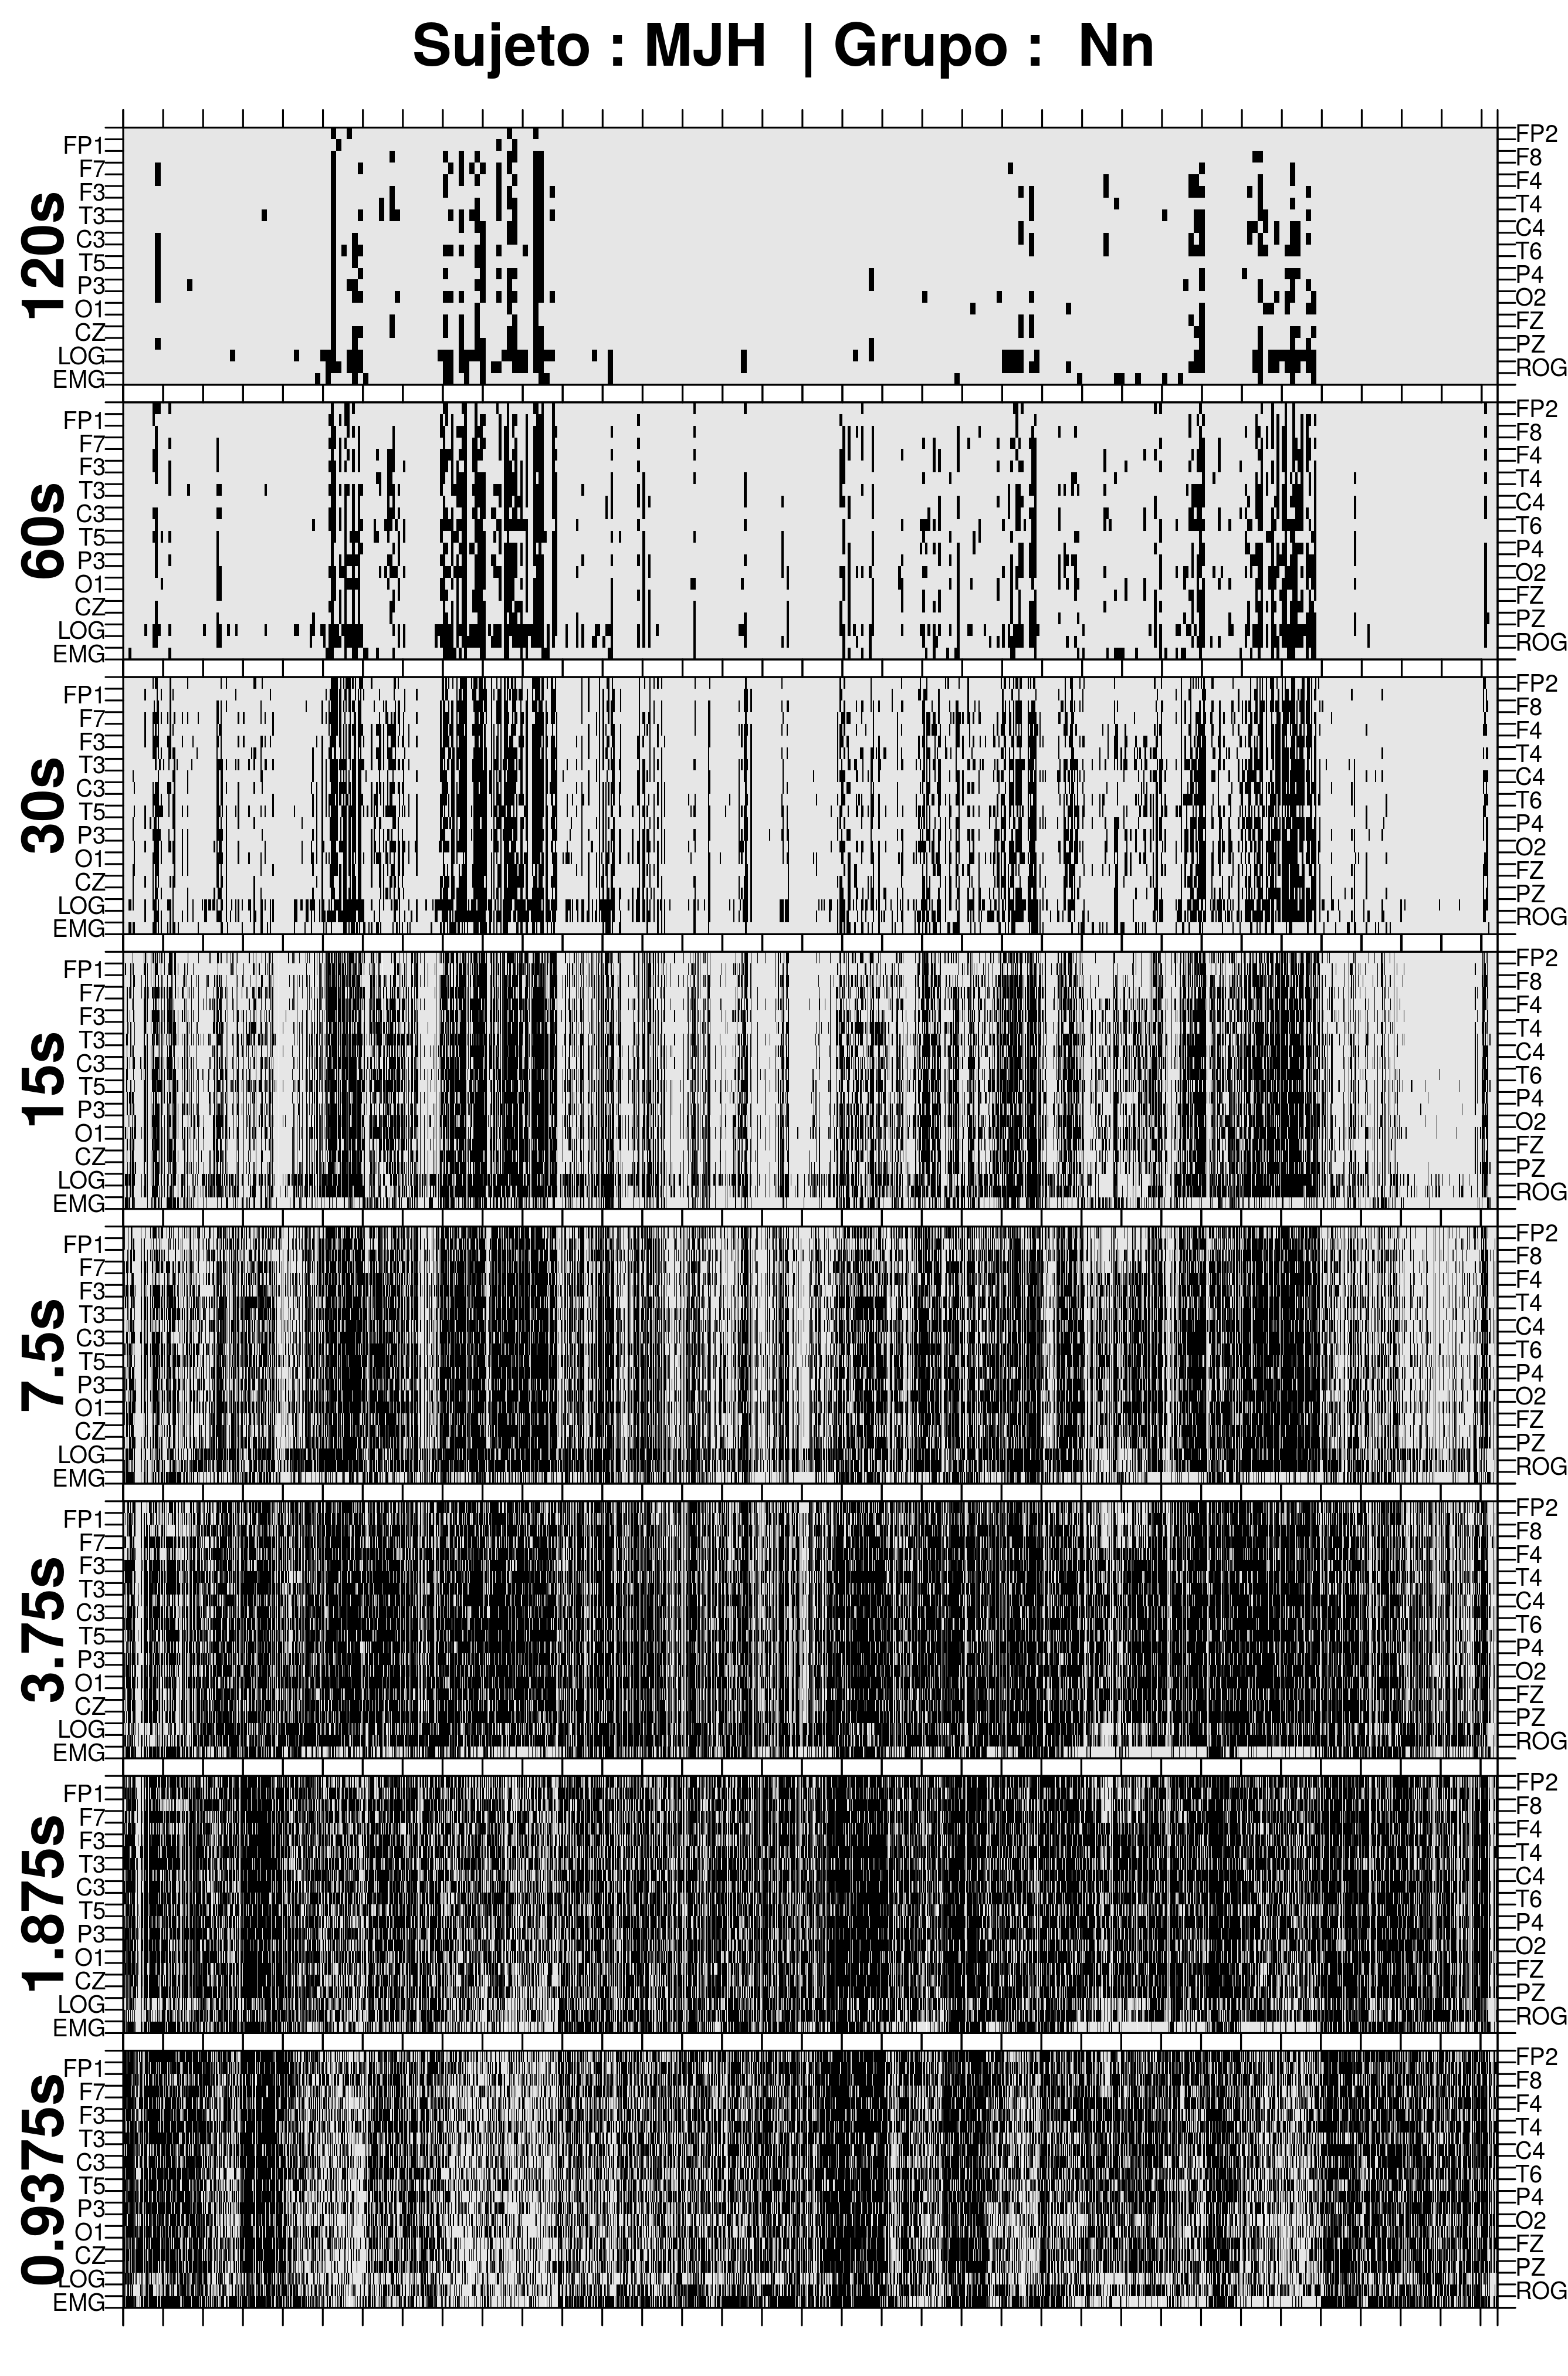
\includegraphics[width=0.9\linewidth]
{./img_ejemplos/MJNNVIGILOS_comp_est_.png} 
\end{figure}

\begin{figure}
\centering
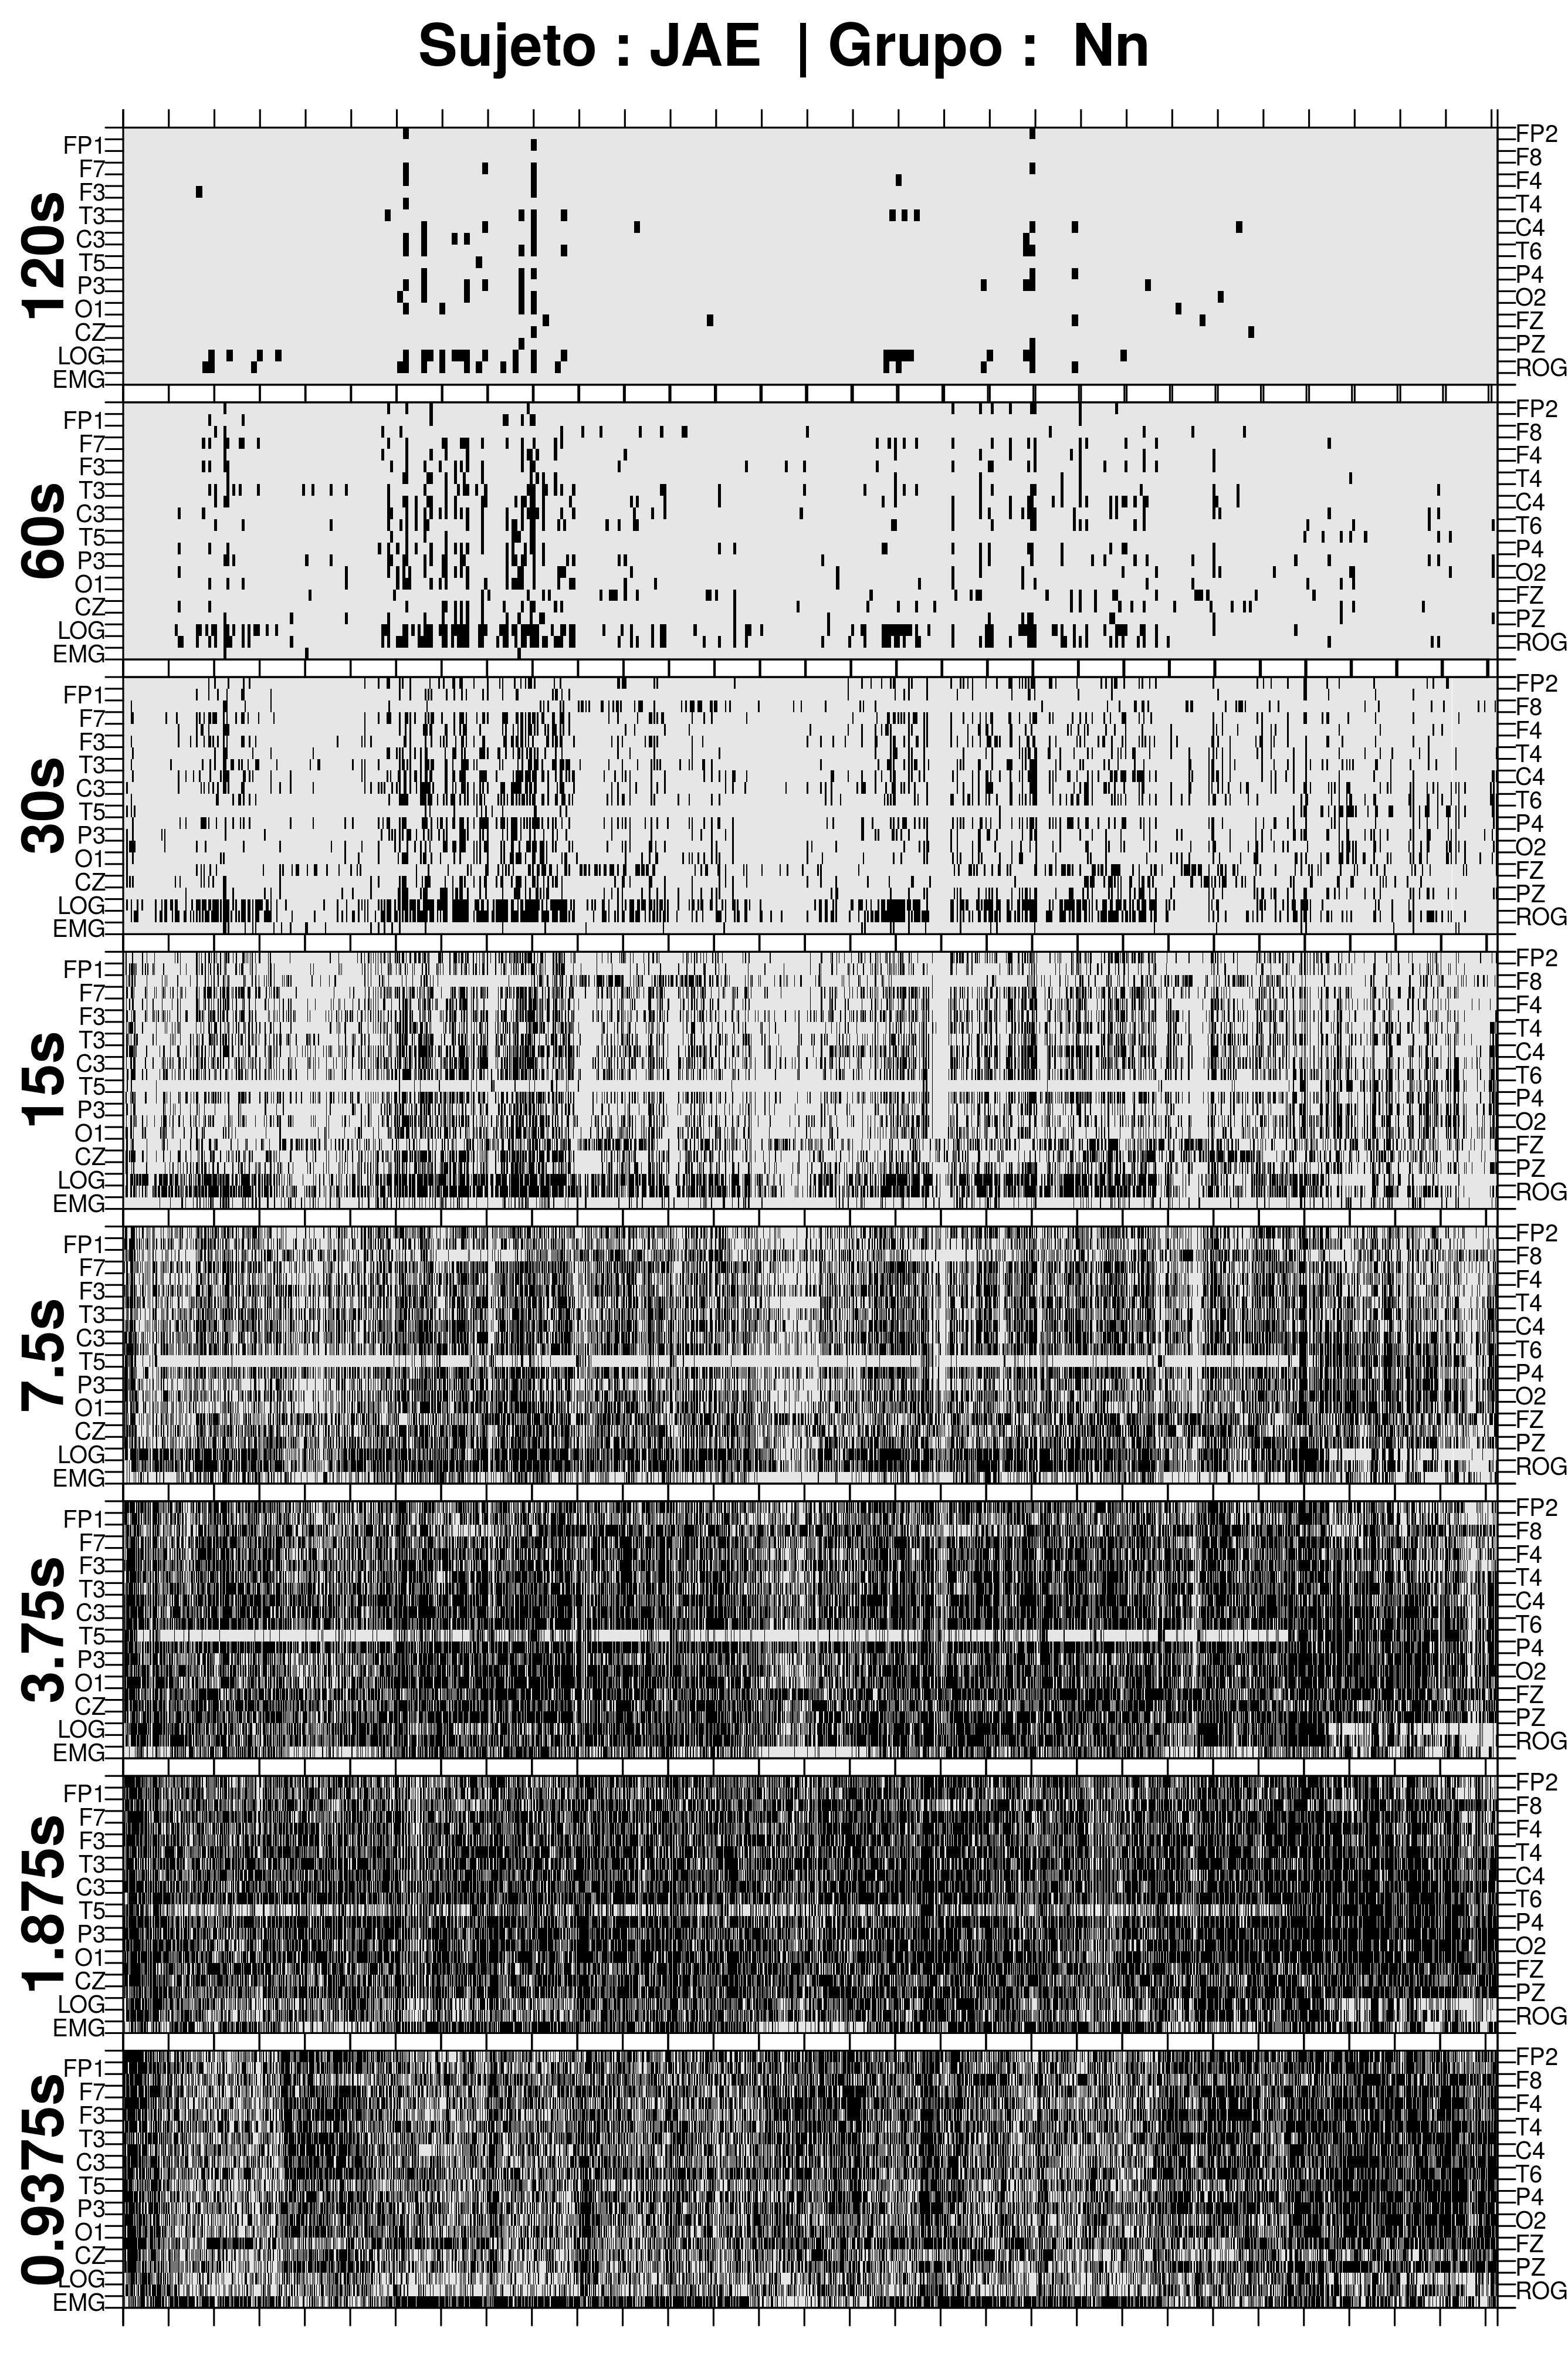
\includegraphics[width=0.9\linewidth]
{./img_ejemplos/JANASUE_comp_est_.png} 
\end{figure}

\begin{figure}
\centering
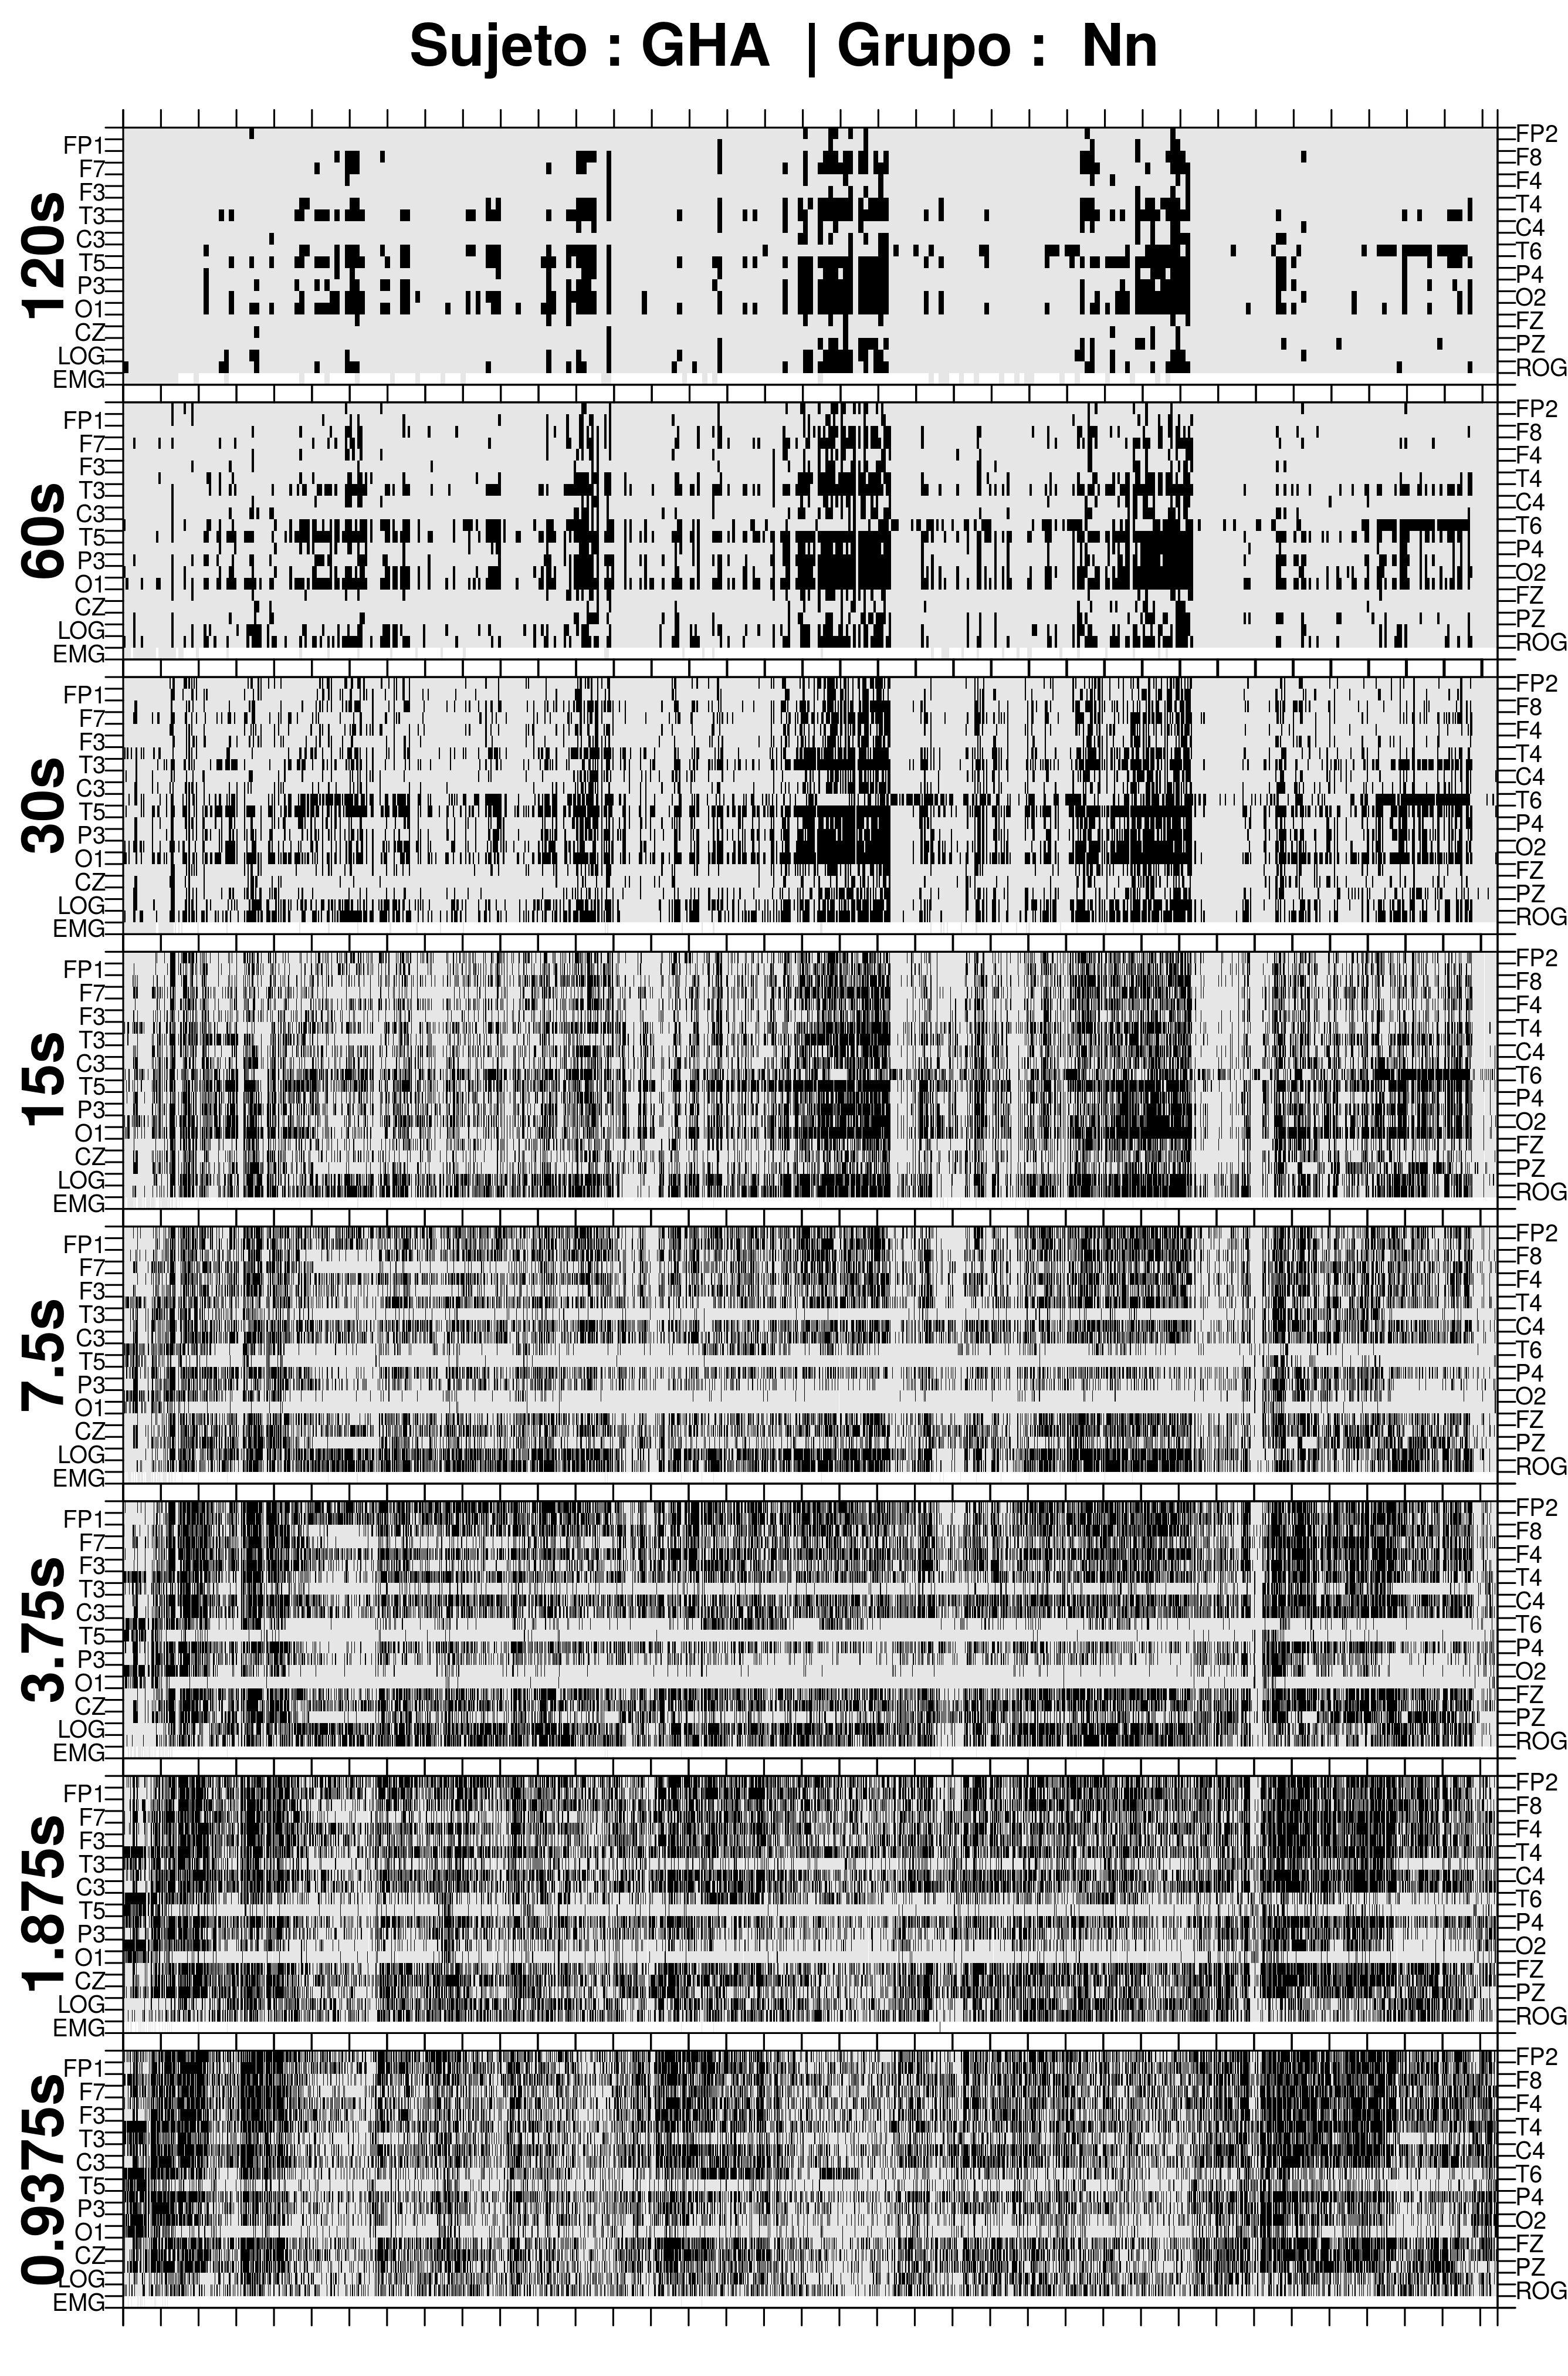
\includegraphics[width=0.9\linewidth]
{./img_ejemplos/GH24031950SUENO_comp_est_.png} 
\end{figure}

\begin{figure}
\centering
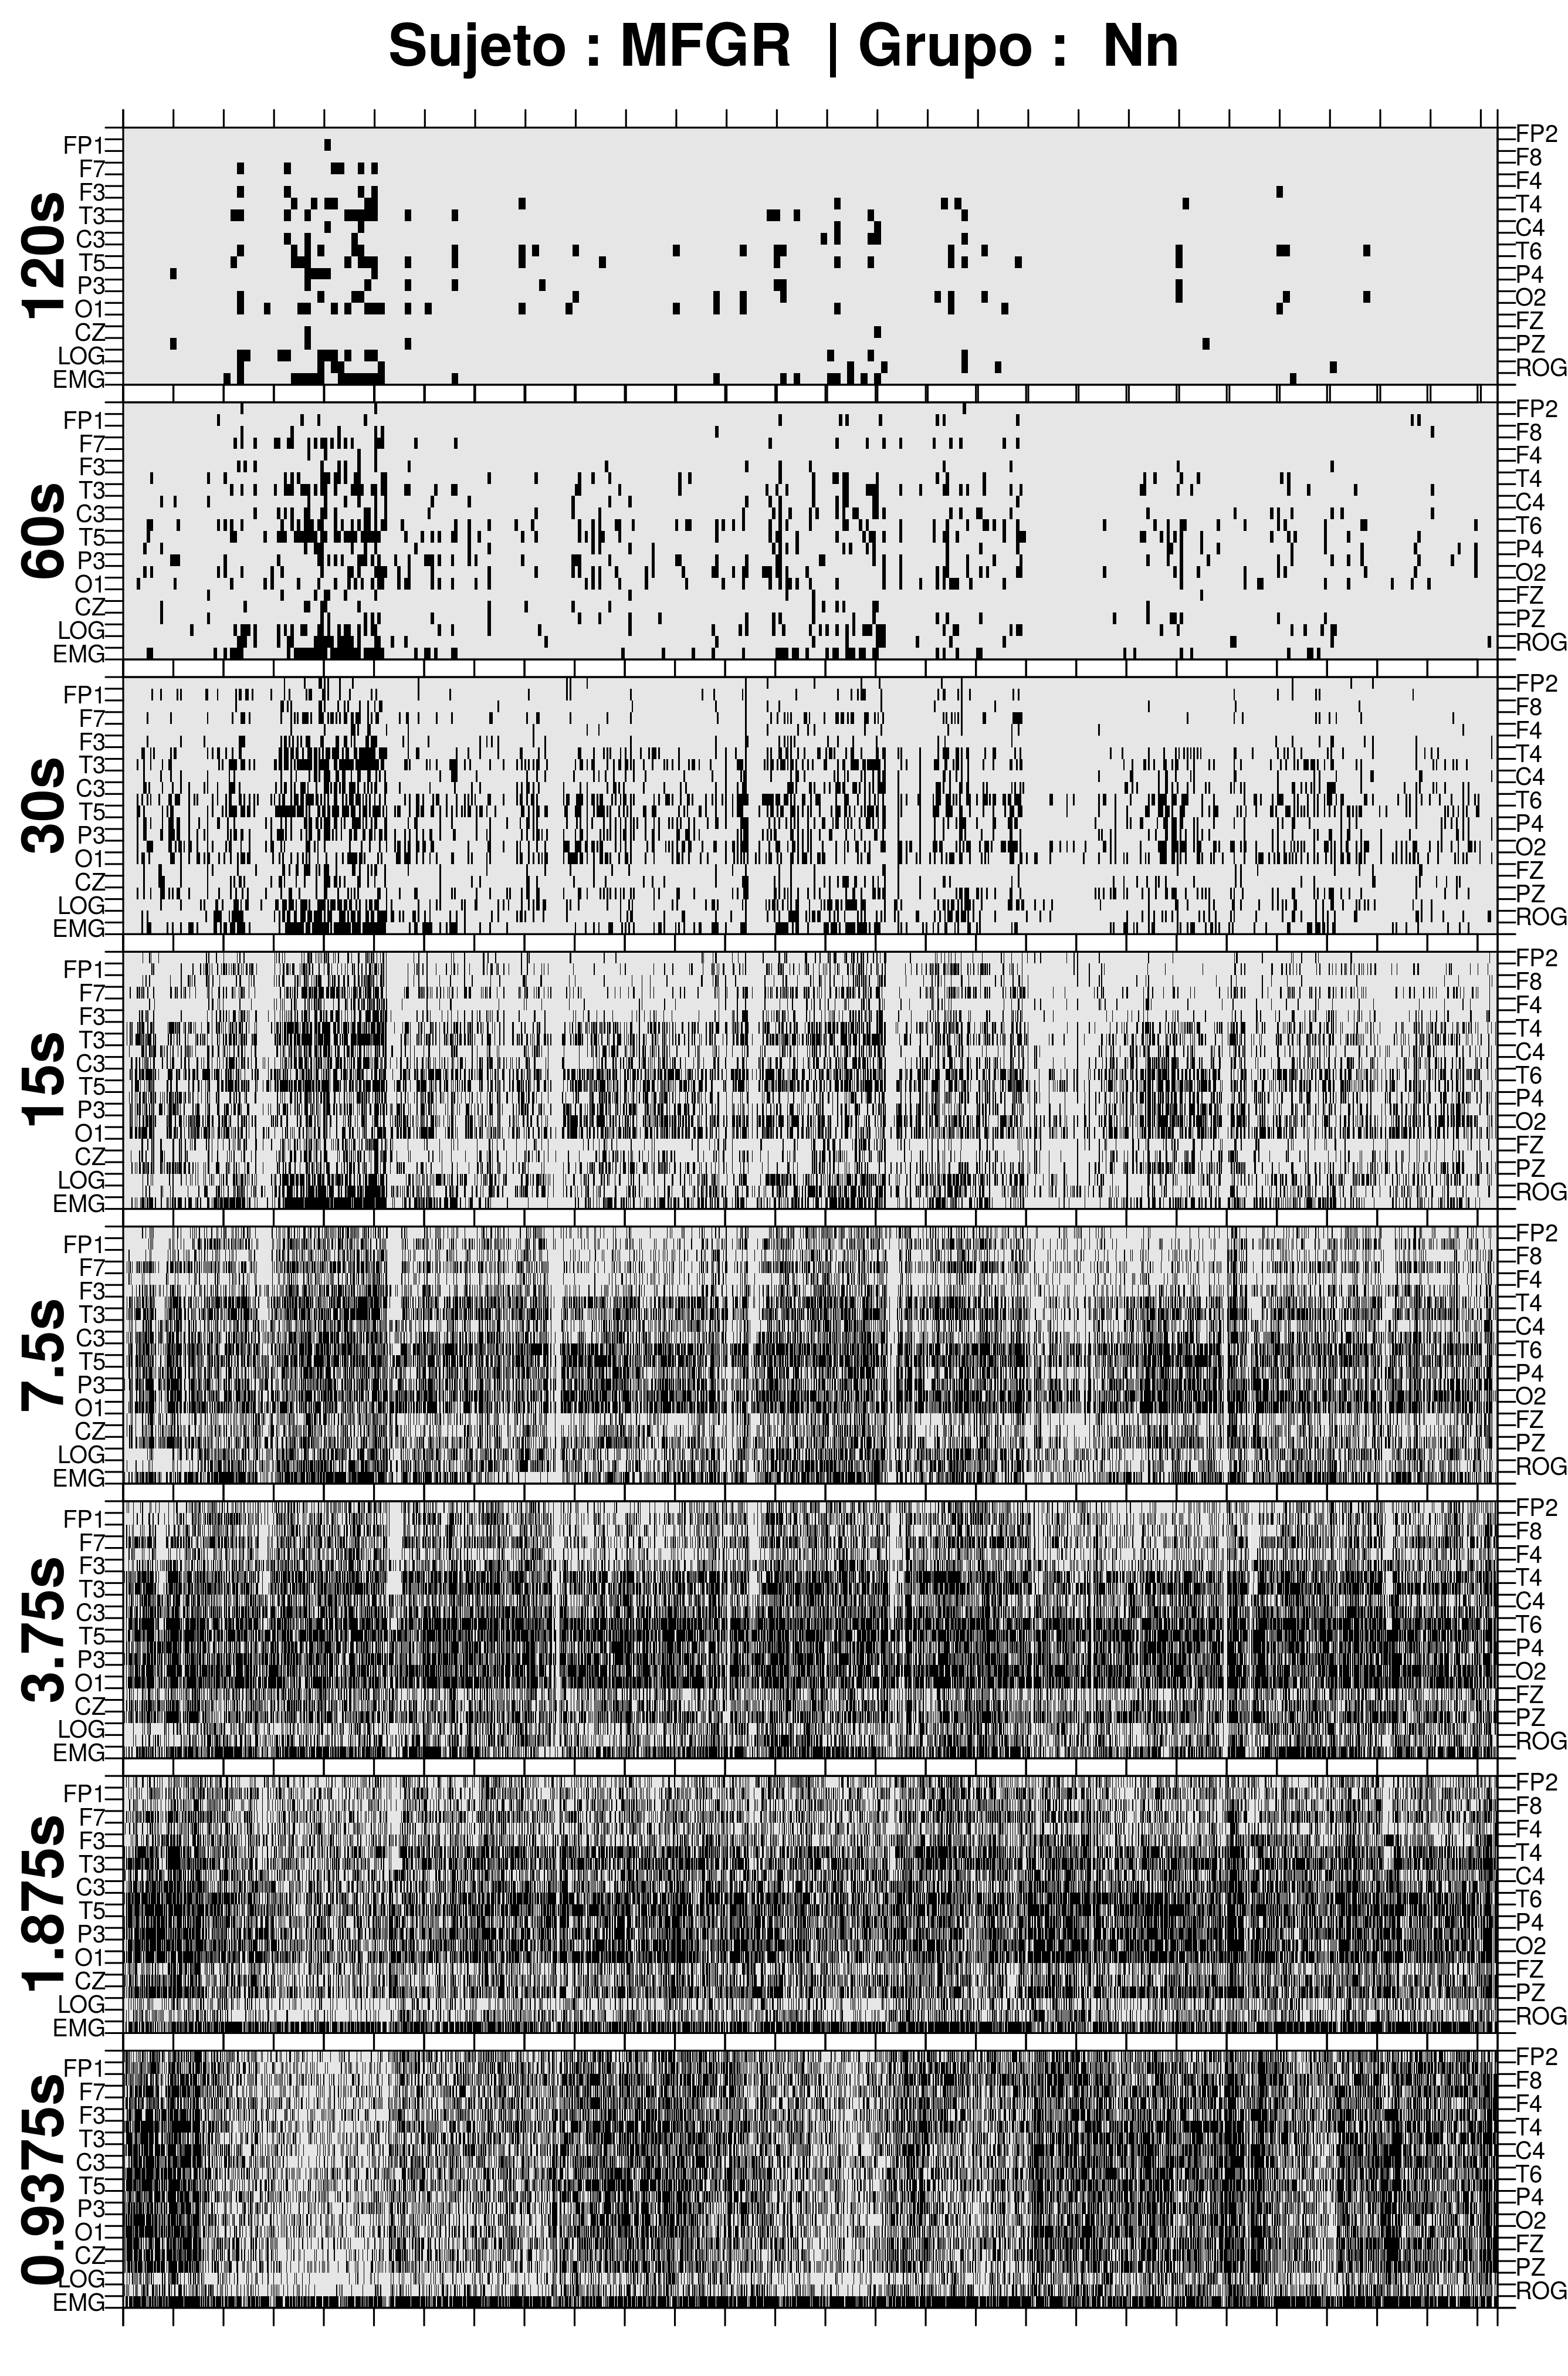
\includegraphics[width=0.9\linewidth]
{./img_ejemplos/GURM251148SUE_comp_est_.png} 
\end{figure}

%%%%%%%%%%%%%%%%%%%%%%%%%%%%%%%%%%%%%

\begin{figure}
\centering
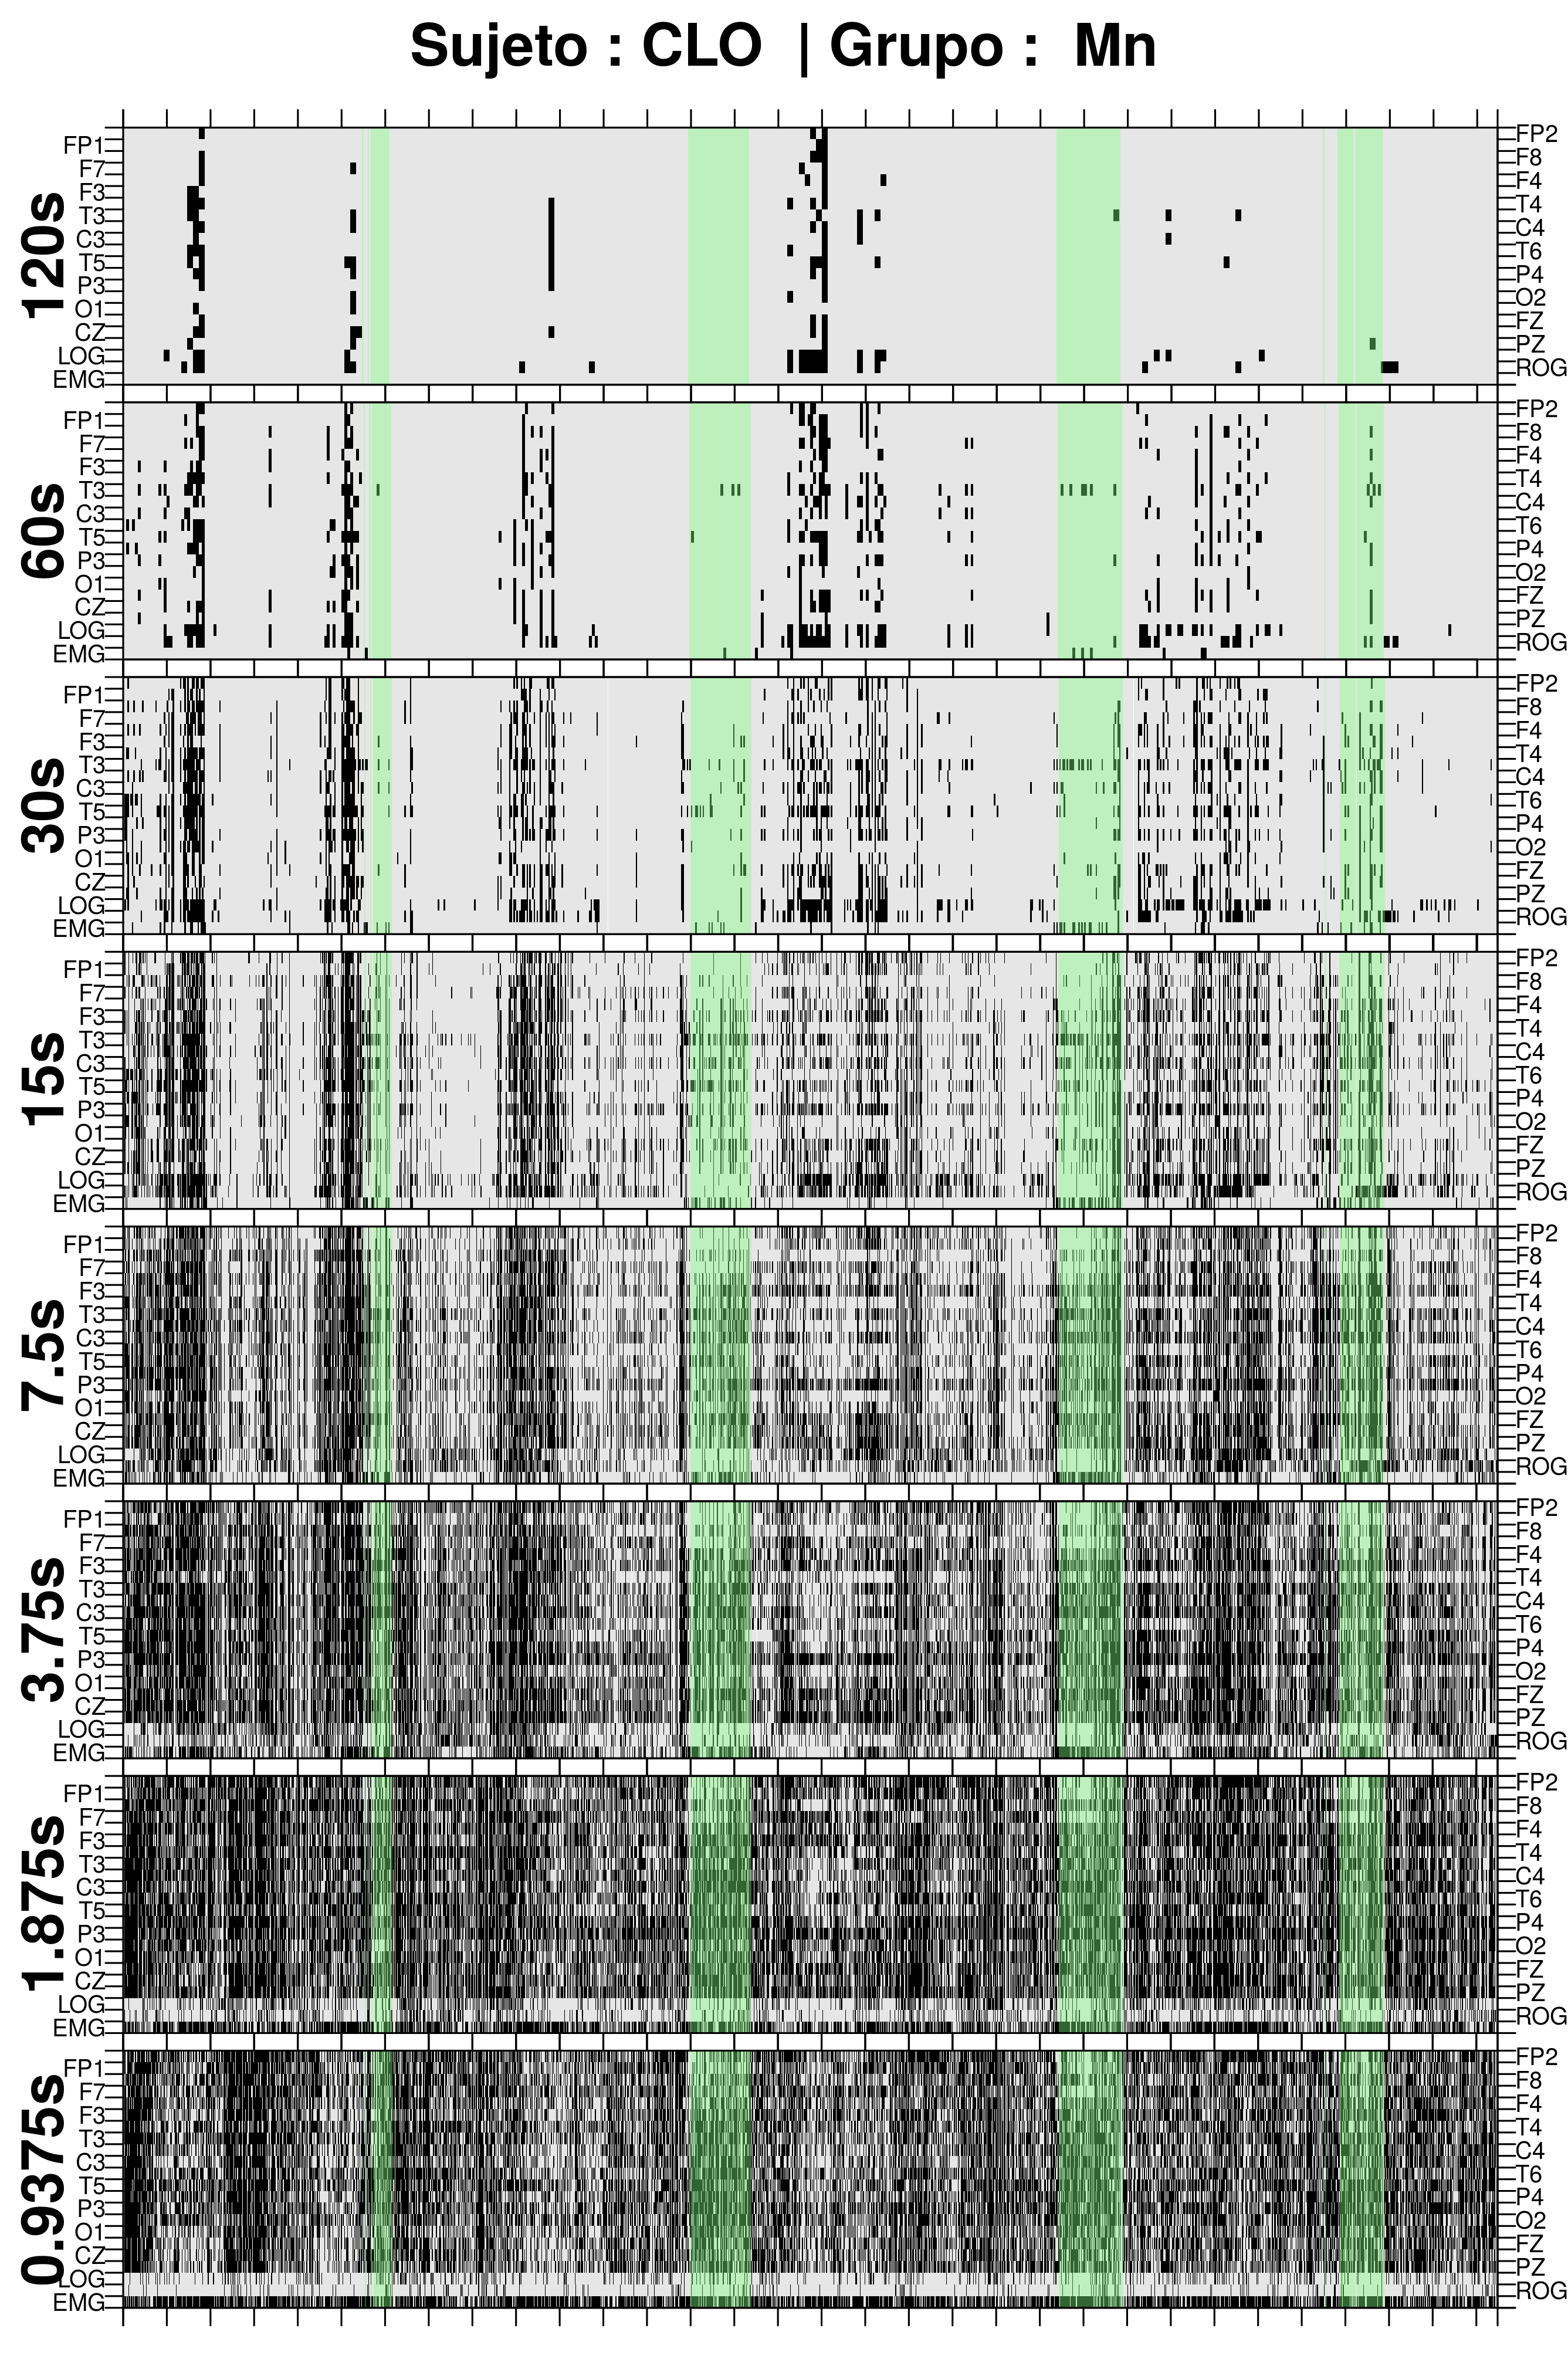
\includegraphics[width=0.9\linewidth]
{./img_ejemplos/CLMN10SUE_comp_est_.png} 
\end{figure}

\begin{figure}
\centering
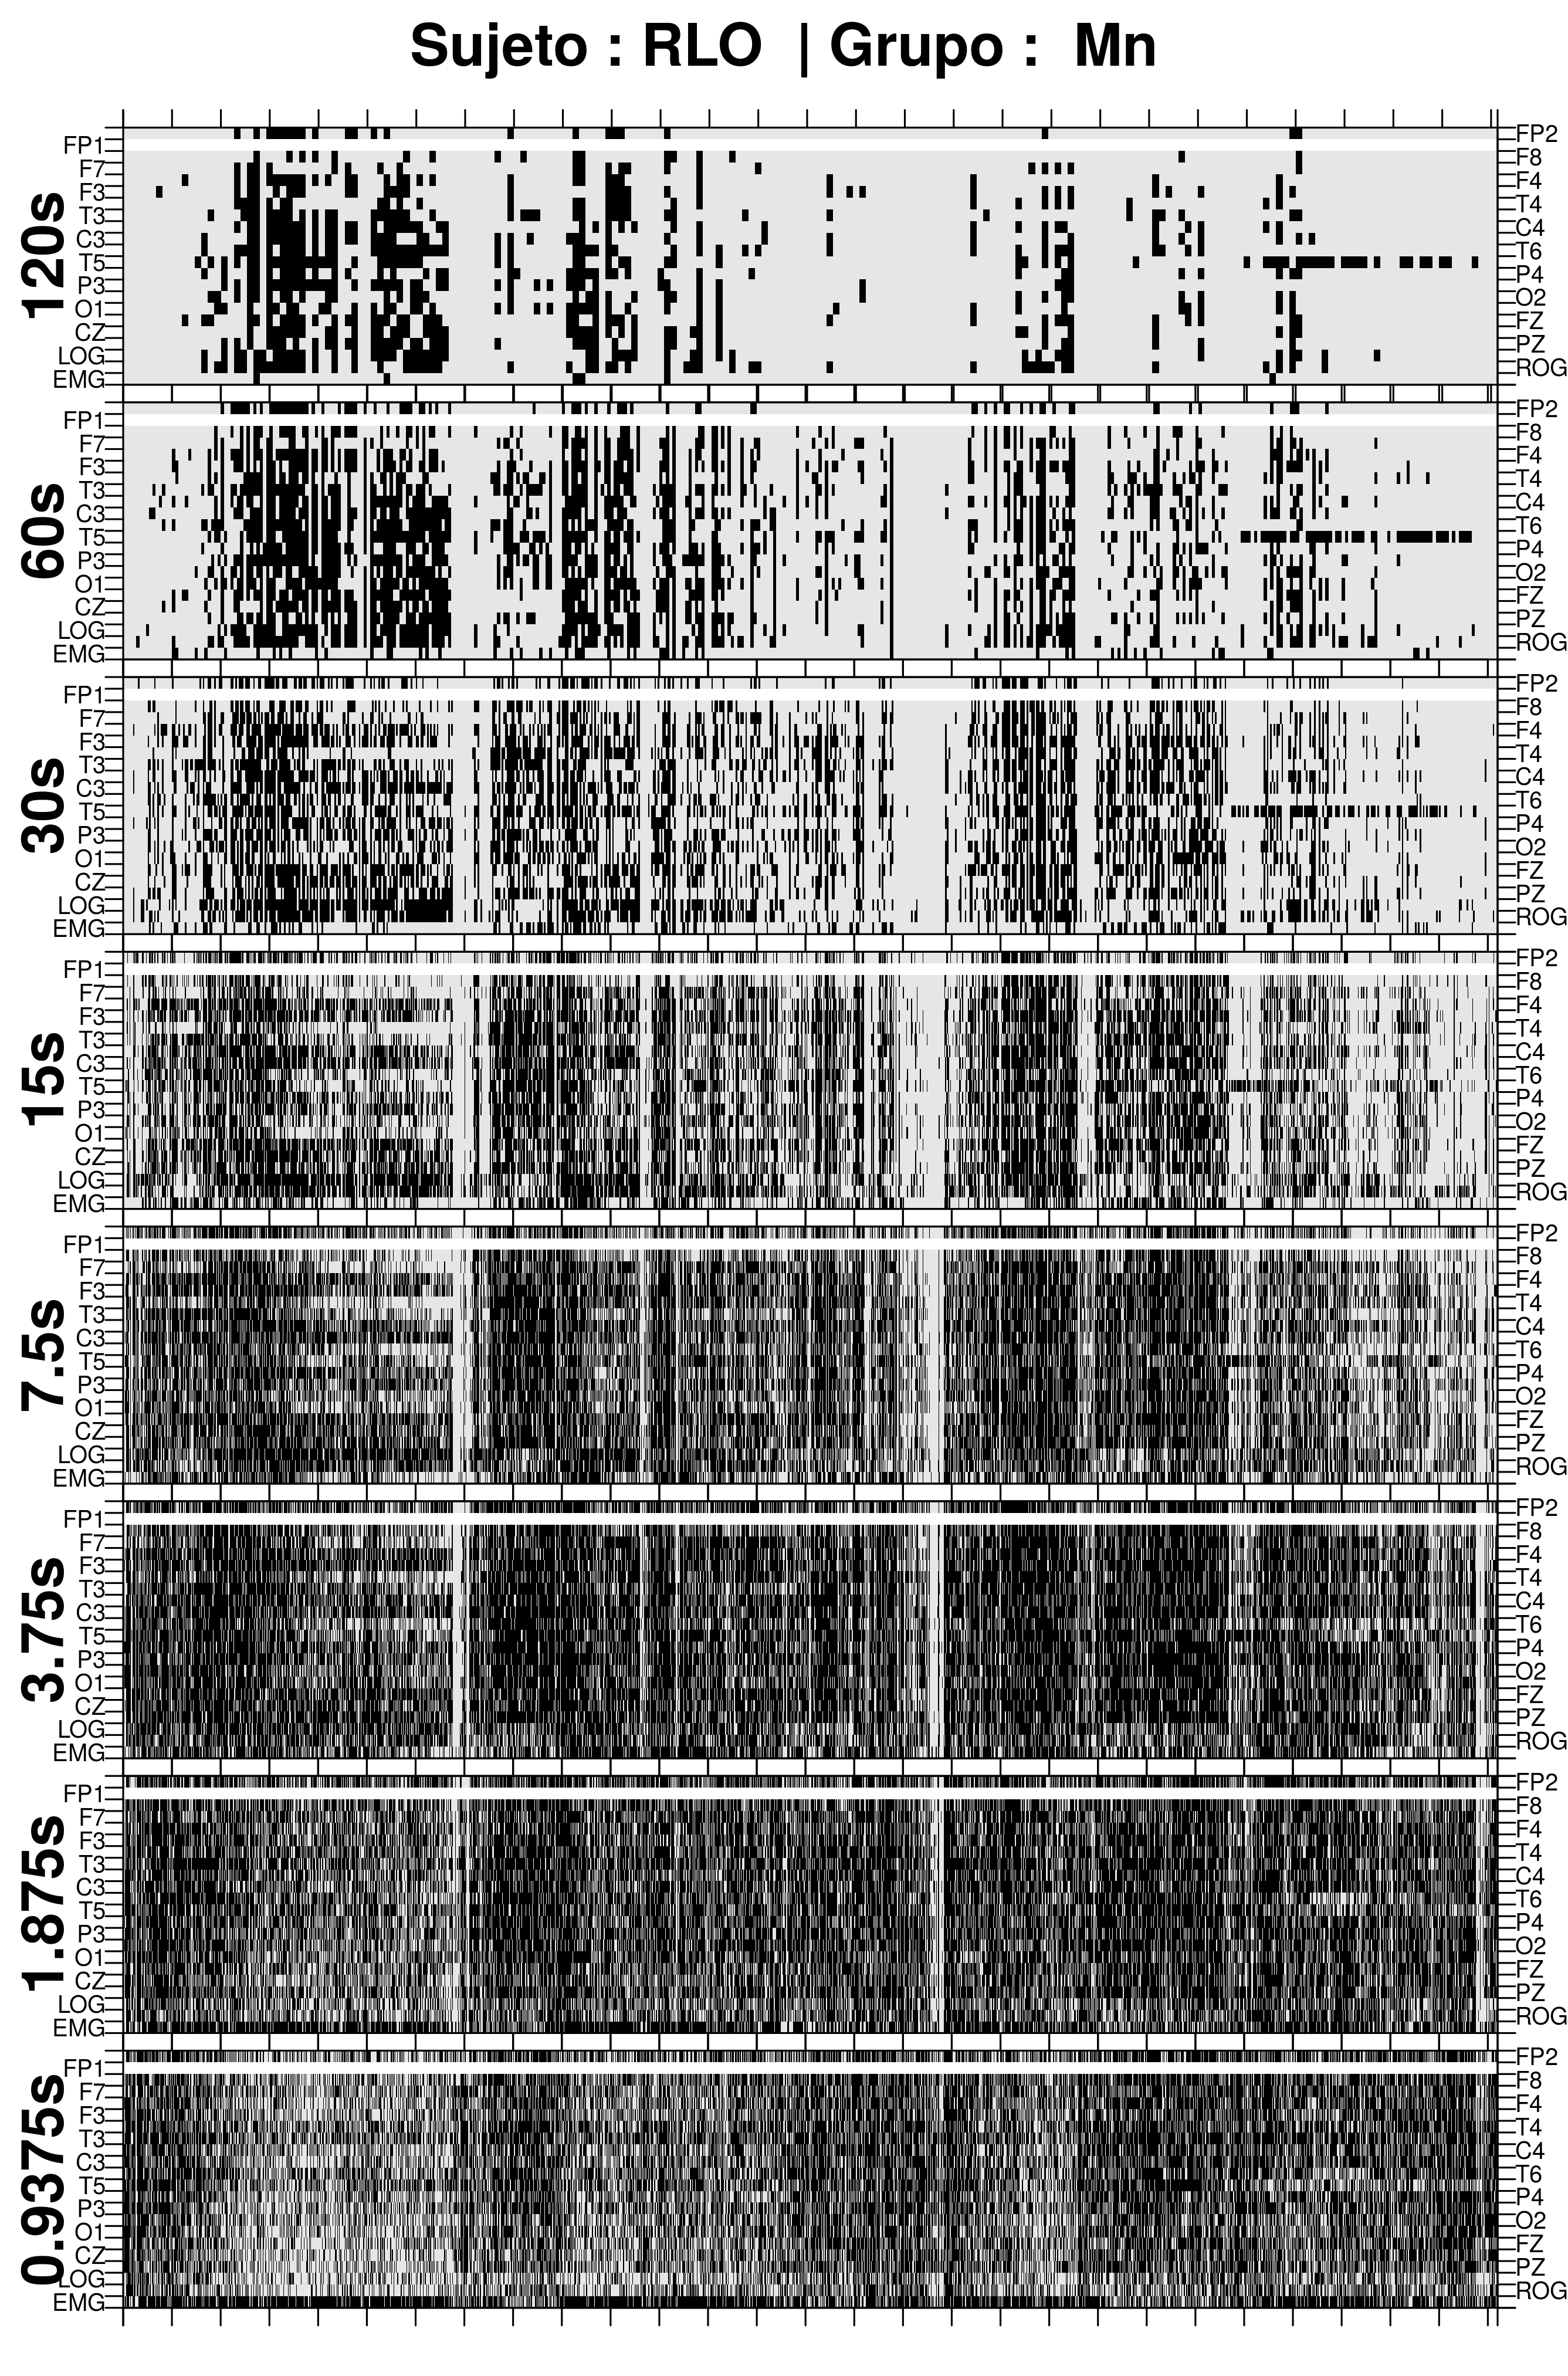
\includegraphics[width=0.9\linewidth]
{./img_ejemplos/RLMN10SUE_comp_est_.png} 
\end{figure}

\begin{figure}
\centering
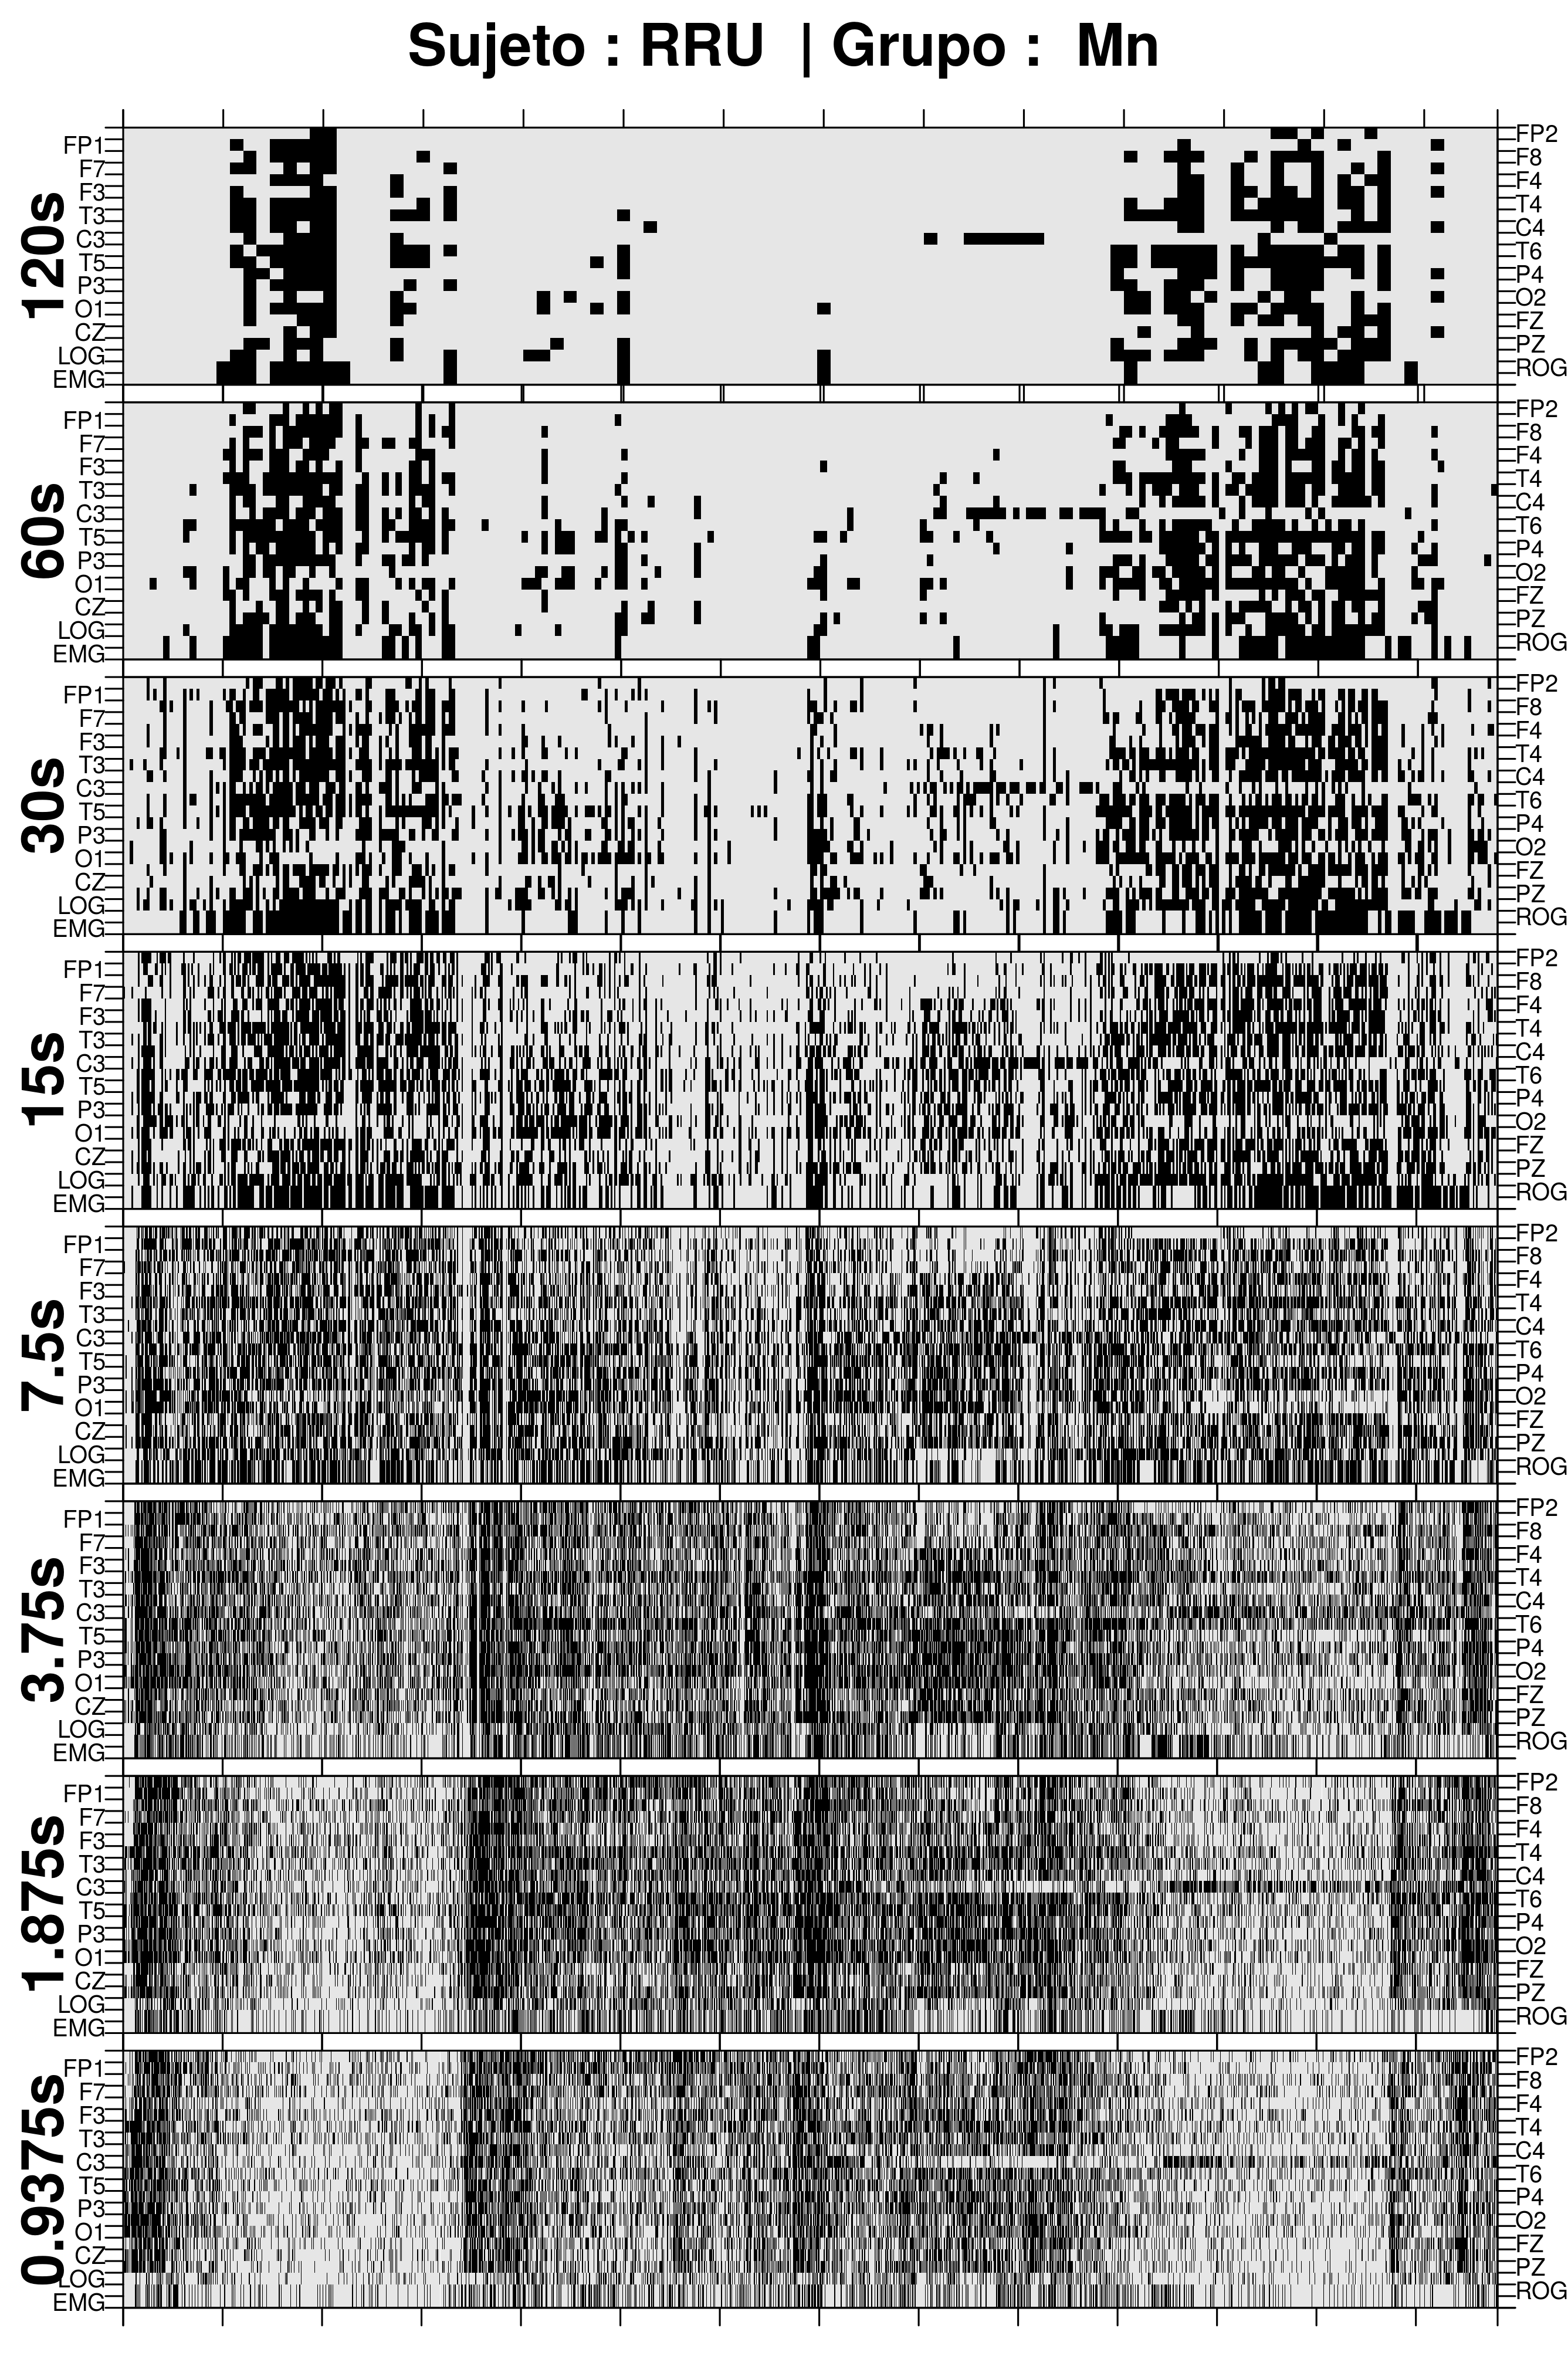
\includegraphics[width=0.9\linewidth]
{./img_ejemplos/RRMNS_comp_est_.png} 
\end{figure}

%%%%%%%%%%%%%%%%%%%%%%%%%%%%%%%%%%%%%%%%%%%%%%%%%
%%%%%%%%%%%%%%%%%%%%%%%%%%%%%%%%%%%%%%%%%%%%%%%%%

\begin{figure}
\bordes{1.5}
\begin{tabular}{l}
\Large{{Patrones visuales}}\\
\begin{tabular}{c}
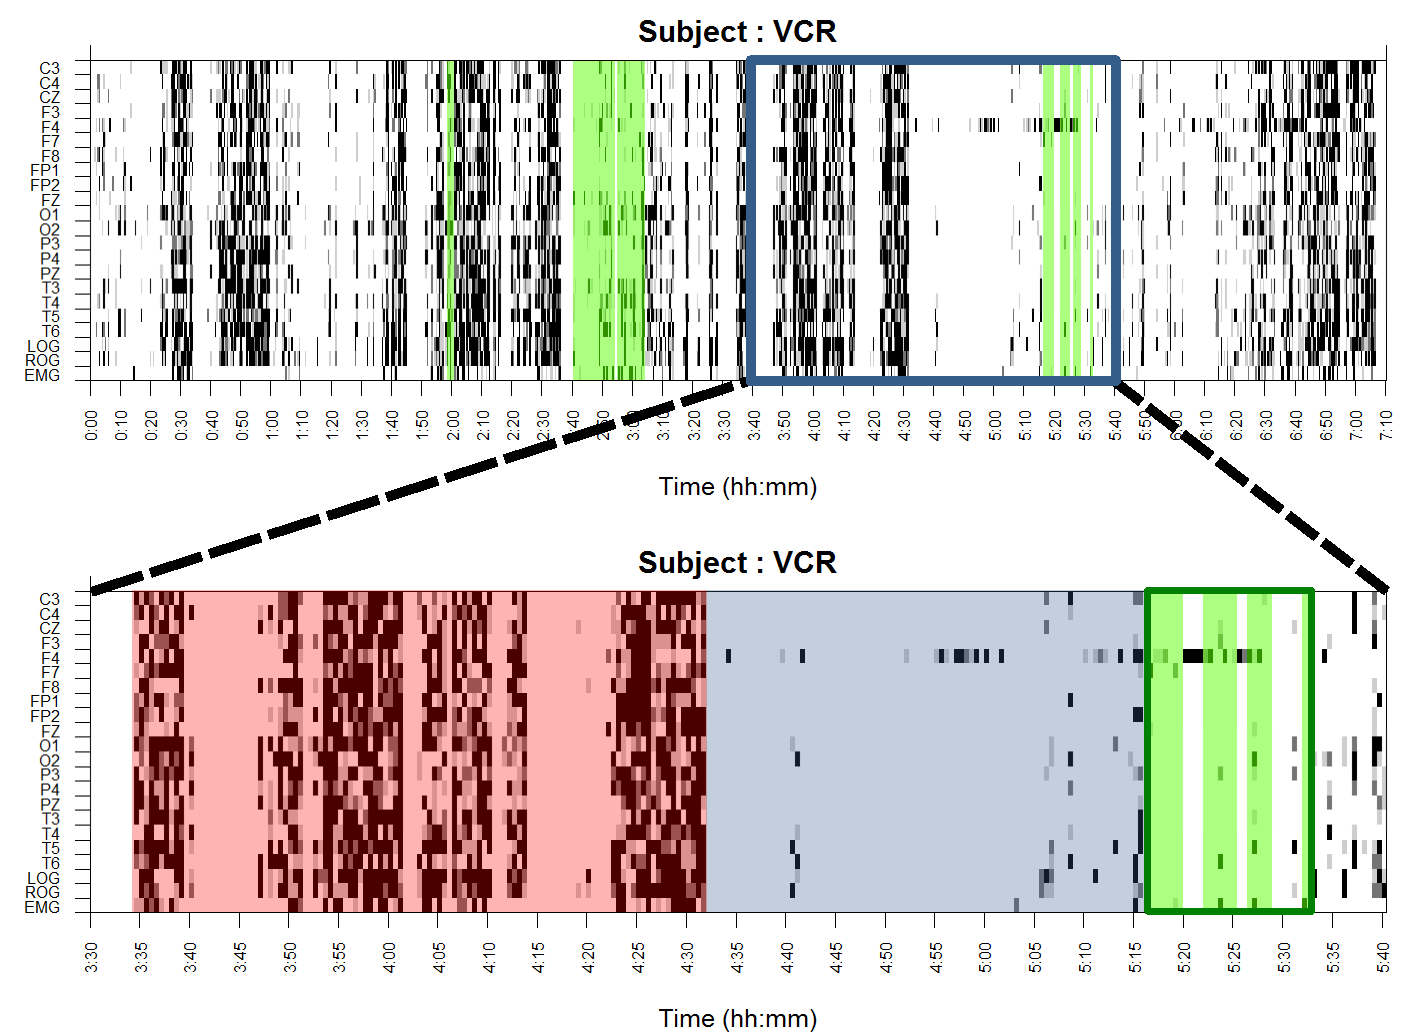
\includegraphics[width=0.45\textwidth]
{./img_ejemplos/zoom_VCR.pdf}
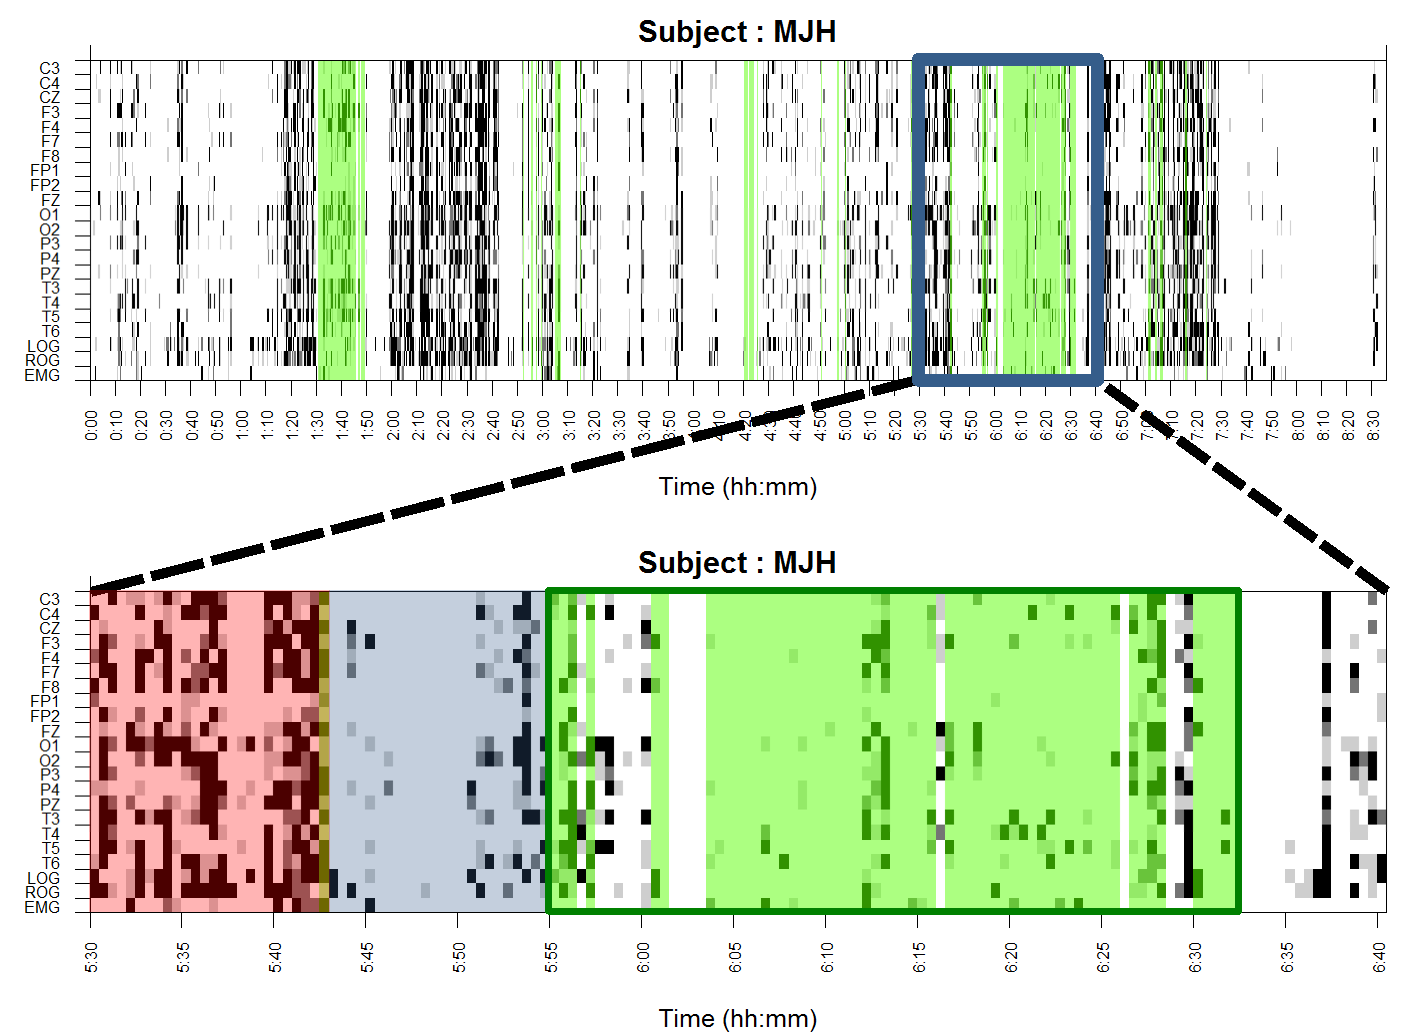
\includegraphics[width=0.45\textwidth]
{./img_ejemplos/zoom_MJH.pdf}
\\
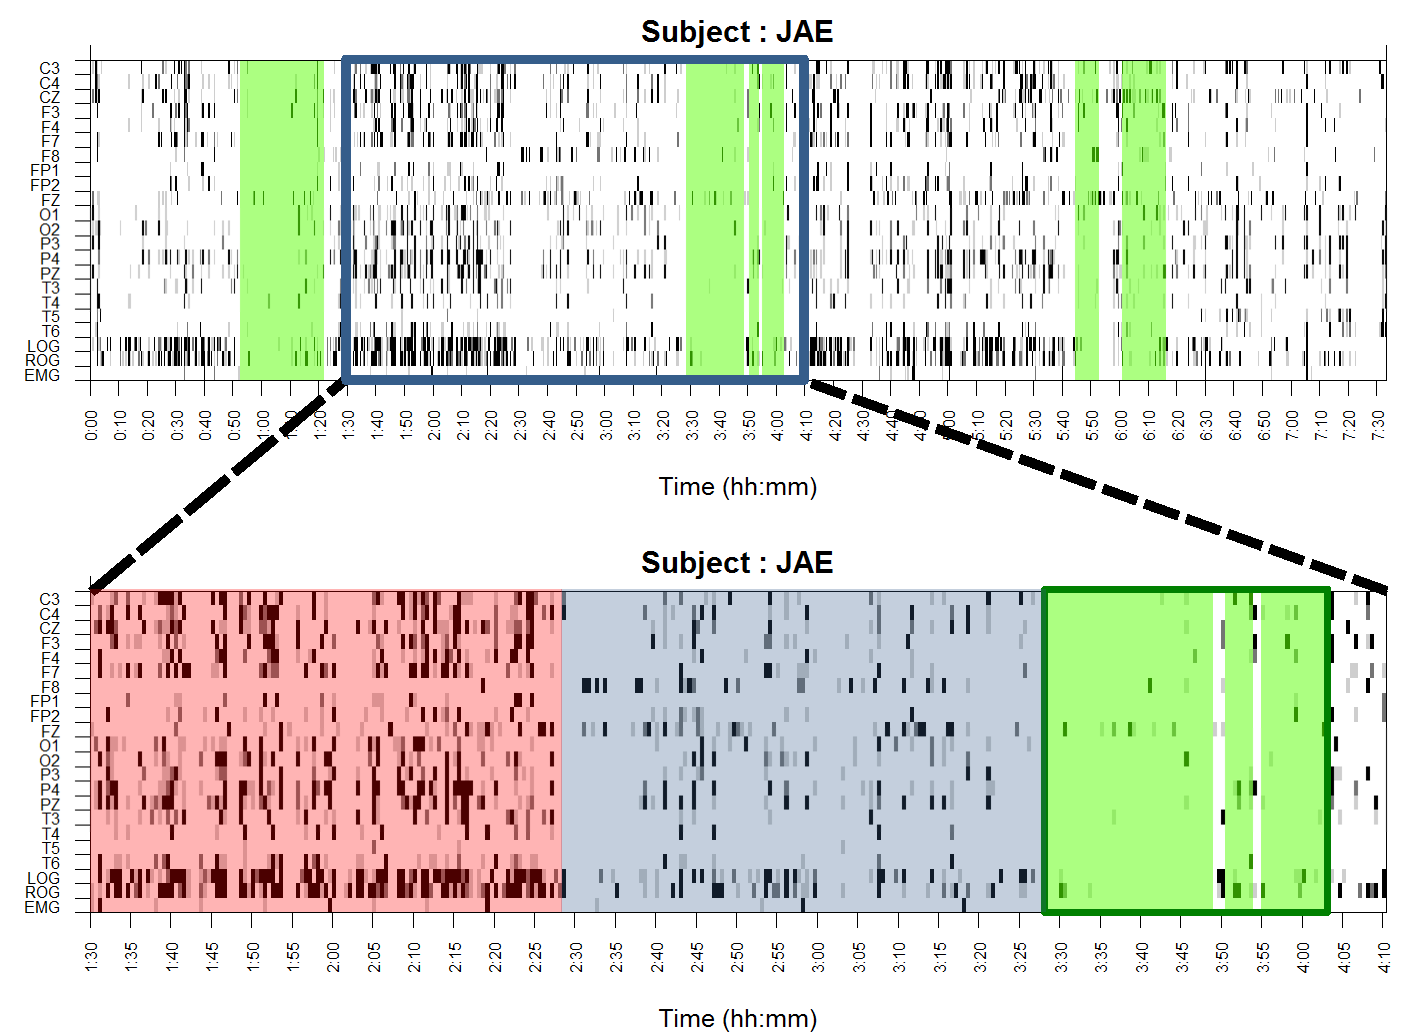
\includegraphics[width=0.45\textwidth]
{./img_ejemplos/zoom_JAE.pdf}
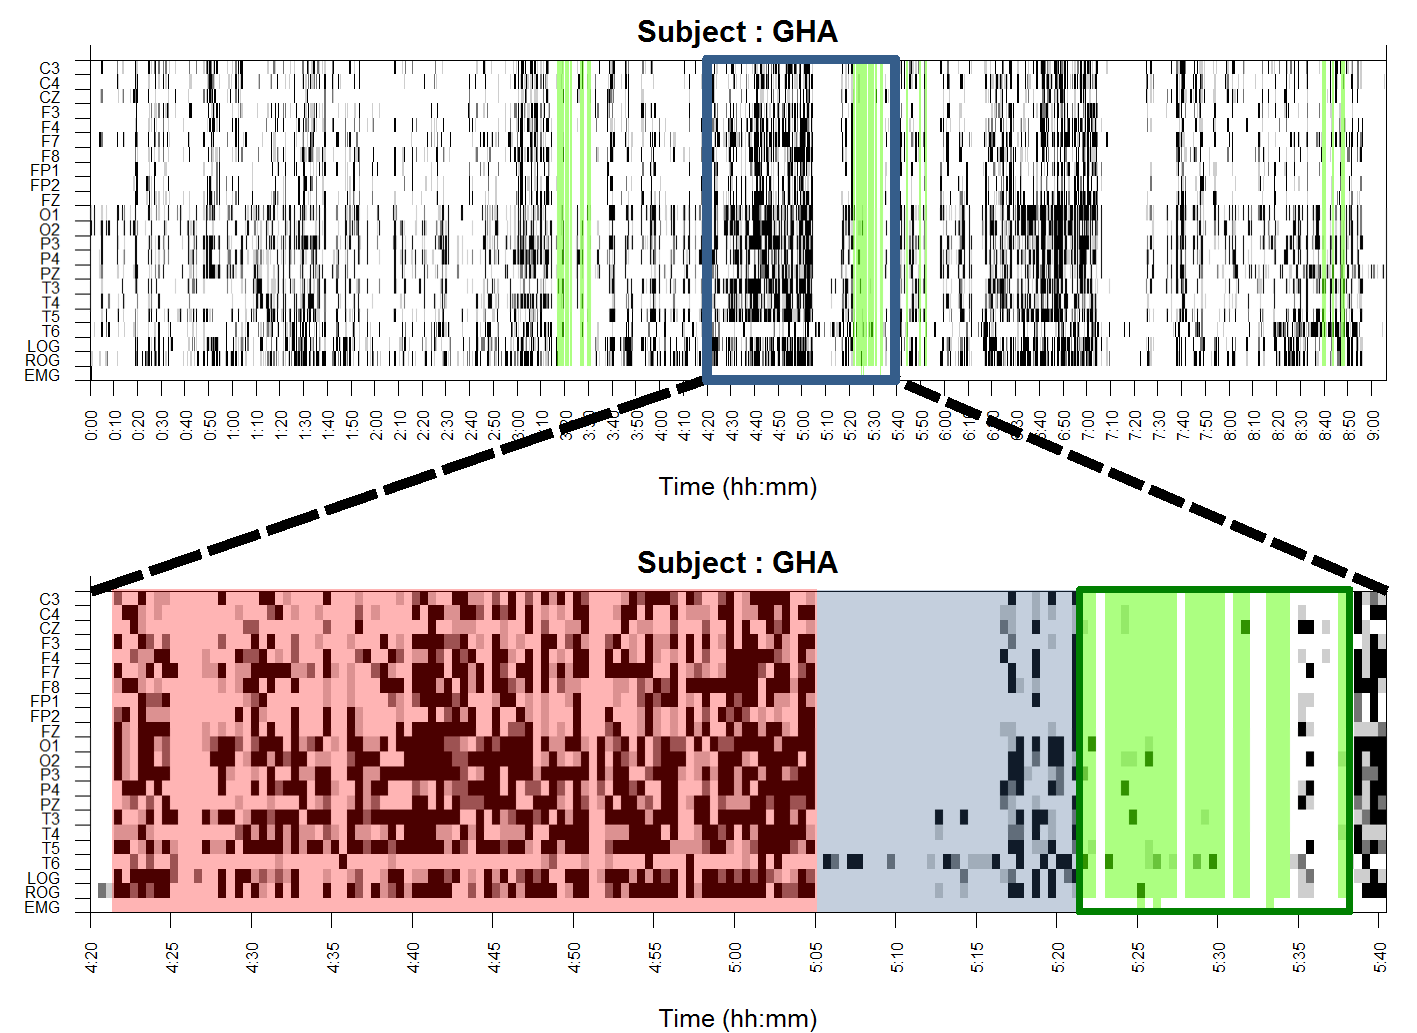
\includegraphics[width=0.45\textwidth]
{./img_ejemplos/zoom_GHA.pdf}
\\
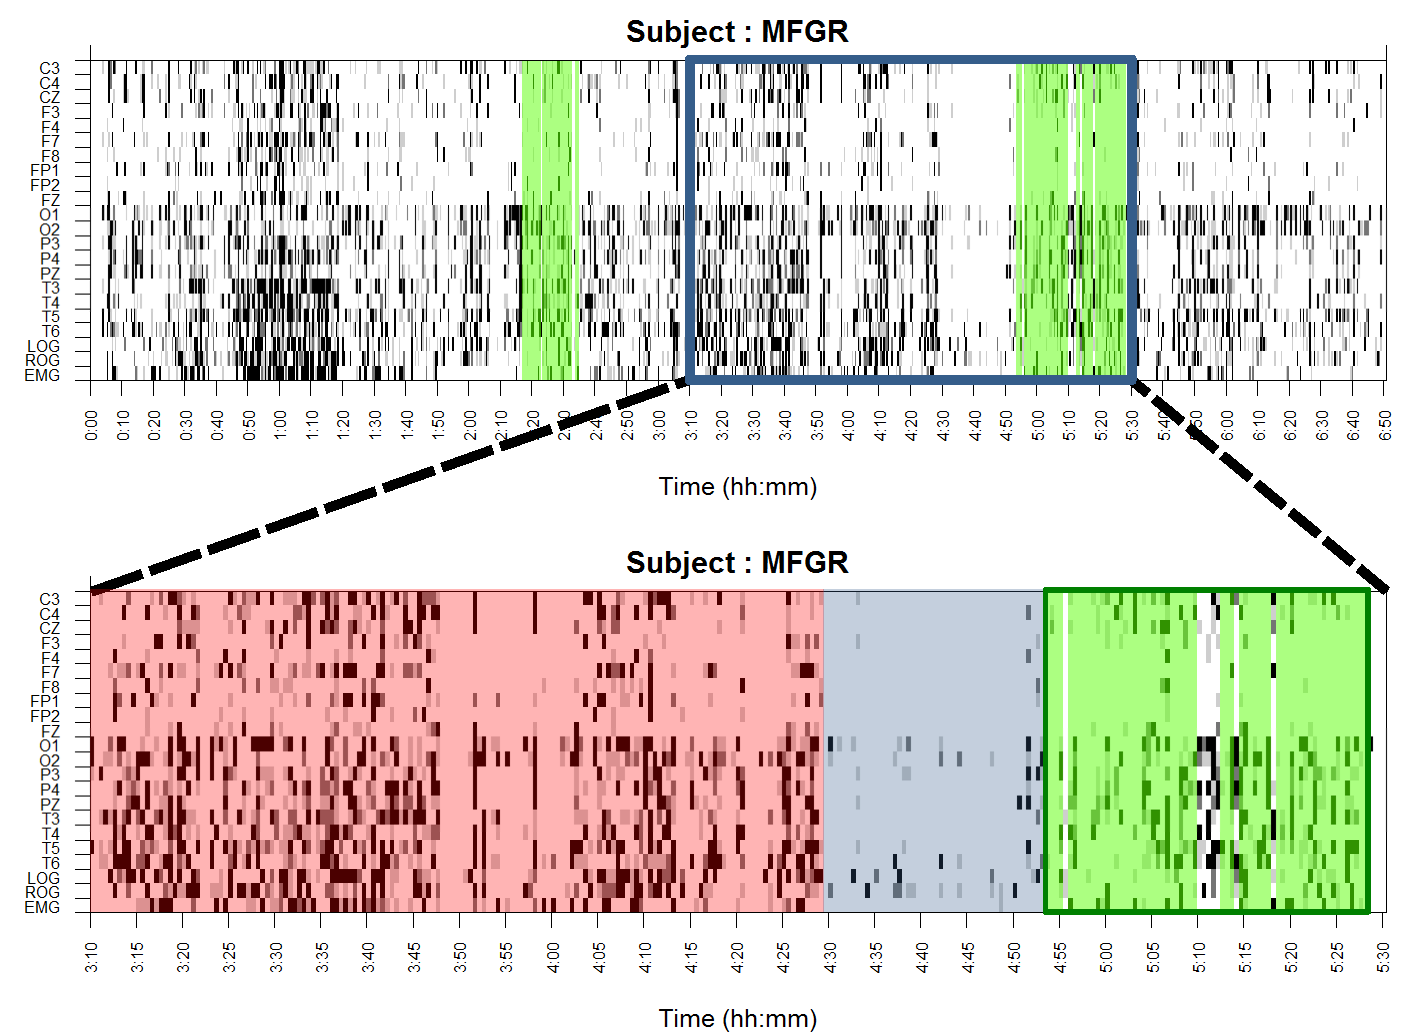
\includegraphics[width=0.45\textwidth]
{./img_ejemplos/zoom_MFGR.pdf}
\end{tabular}
\end{tabular}
\end{figure}

%%%%%%%%%%%%%%%%%%%%%%%%%%%%%%%%%%%%%%%%%%%%%%%%%%%%%%%%%%%%%%%%%%%%%%%%%%%%%%%%%%%%%%%%%%%%%%%%%%%
%%%%%%%%%%%%%%%%%%%%%%%%%%%%%%%%%%%%%%%%%%%%%%%%%%%%%%%%%%%%%%%%%%%%%%%%%%%%%%%%%%%%%%%%%%%%%%%%%%%
%%%%%%%%%%%%%%%%%%%%%%%%%%%%%%%%%%%%%%%%%%%%%%%%%%%%%%%%%%%%%%%%%%%%%%%%%%%%%%%%%%%%%%%%%%%%%%%%%%%
%%%%%%%%%%%%%%%%%%%%%%%%%%%%%%%%%%%%%%%%%%%%%%%%%%%%%%%%%%%%%%%%%%%%%%%%%%%%%%%%%%%%%%%%%%%%%%%%%%%
